\documentclass{beamer}
    \usepackage[utf8]{inputenc}
    \usepackage[russian]{babel}
    \usepackage{amsmath, mathrsfs, mathtext}
    \usepackage{amsfonts}
    \usepackage{graphicx, epsfig}
    \usepackage{subcaption}
    \captionsetup[subfigure]{labelformat=empty}
    \usetheme{Warsaw}%{Singapore}%{Warsaw}%{Warsaw}%{Darmstadt}
    \usecolortheme{sidebartab}
    \usepackage{bbm}
    \newcommand{\bz}{\mathbf{z}}
\newcommand{\bx}{\mathbf{x}}
\newcommand{\by}{\mathbf{y}}
\newcommand{\bw}{\mathbf{w}}
\newcommand{\bY}{\mathbf{Y}}
\newcommand{\bX}{\mathbf{X}}
\newcommand{\ba}{\mathbf{a}}
\newcommand{\bu}{\mathbf{u}}
\newcommand{\bt}{\mathbf{t}}
\newcommand{\bp}{\mathbf{p}}
\newcommand{\bq}{\mathbf{q}}
\newcommand{\br}{\mathbf{r}}
\newcommand{\bg}{\mathbf{g}}
\newcommand{\bh}{\mathbf{h}}
\newcommand{\bb}{\mathbf{b}}
\newcommand{\bv}{\mathbf{v}}
\newcommand{\be}{\mathbf{e}}
\newcommand{\bc}{\mathbf{c}}
\newcommand{\bs}{\mathbf{s}}
\newcommand{\bP}{\mathbf{P}}
\newcommand{\bT}{\mathbf{T}}
\newcommand{\bQ}{\mathbf{Q}}
\newcommand{\bE}{\mathbf{E}}
\newcommand{\bF}{\mathbf{F}}
\newcommand{\bU}{\mathbf{U}}
\newcommand{\bI}{\mathbf{I}}
\newcommand{\bB}{\mathbf{B}}
\newcommand{\bW}{\mathbf{W}}
\newcommand{\bD}{\mathbf{D}}
\newcommand{\bH}{\mathbf{H}}
\newcommand{\bG}{\mathbf{G}}
\newcommand{\bS}{\mathbf{S}}
\newcommand{\bZ}{\mathbf{Z}}
\newcommand{\bJ}{\mathbf{J}}
\newcommand{\bM}{\mathbf{M}}
\newcommand{\btheta}{\boldsymbol{\theta}}
\newcommand{\bmu}{\boldsymbol{\mu}}
\newcommand{\blambda}{\boldsymbol{\lambda}}
\newcommand{\bPsi}{\boldsymbol{\Psi}}
\newcommand{\bchi}{\boldsymbol{\chi}}
\newcommand{\bsigma}{\boldsymbol{\sigma}}
\newcommand{\bTheta}{\boldsymbol{\Theta}}
\newcommand{\bphi}{\boldsymbol{\phi}}
\newcommand{\bdelta}{\boldsymbol{\delta}}

\newcommand{\brs}[1]{\left(#1\right)}
\newcommand{\sbrs}[1]{\left[#1\right]}
\newcommand{\fbrs}[1]{\left\{#1\right\}}
\newcommand{\rbrs}[1]{\left\langle #1 \right\rangle}

\newcommand{\R}{\mathbb{R}}
\newcommand{\Q}{\mathbb{Q}}
\renewcommand{\C}{\mathbb{C}}
\newcommand{\N}{\mathbb{N}}
\newcommand{\Z}{\mathbb{Z}}
\newcommand{\E}{\mathbb{E}}
\newcommand{\var}{\mathrm{Var}\;}
\newcommand{\diam}{\mathrm{diam}\;}
\newcommand{\conv}{\mathrm{conv}\;}
\newcommand{\cl}{\mathrm{cl}\;}
\newcommand{\dist}{\mathbf{dist}}
\newcommand{\dom}{\mathbf{dom}\;}
\newcommand{\sign}{\mathbf{sign}\;}
\newcommand{\T}{\intercal}
\newcommand{\eps}{\varepsilon}
    \DeclareMathOperator*{\argmin}{arg\,min}
    \definecolor{beamer@blendedblue}{RGB}{15,120,80}
    %----------------------------------------------------------------------------------------------------------
    \title[\hbox to 56mm{Ансамбль локальных аппроксимаций\hfill\insertframenumber\,/\,\inserttotalframenumber}]
    {Выбор оптимальных \\ моделей локальной аппроксимации\\ для классификации временных рядов}
    \author[С.\,Д. Иванычев]{\large \\Сергей Дмитриевич Иванычев}
    \institute{\tiny
        Московский физико-технический институт\\
        Физтех-школа прикладной математики и информатики\\
        Факультет управления и прикладной математики\\
        Кафедра <<Интеллектуальные системы>>}

    \date{\footnotesize{Научный руководитель: д.ф.-м.н. В.В.~Стрижов}\\\vspace{\baselineskip}Выпускная квалификационная работа бакалавра\\\vspace{\baselineskip}Москва 2018}
    %----------------------------------------------------------------------------------------------------------
    \begin{document}

    %----------------------------------------------------------------------------------------------------------

    \begin{frame}
    %\thispagestyle{empty}
    \titlepage
    \end{frame}

    %-----------------------------------------------------------------------------------------------------

    \begin{frame}{Классификация временных рядов}

    \vspace{-3 mm}
    \begin{block}{\bf Цель}
   Предложить способ построения набора моделей локальной аппроксимации
   для устойчивой классификации сигналов носимых устройств.
    \end{block}
    \vspace{-3 mm}
    \begin{block}{\bf Гипотеза}
    Суперпозиция моделей локальной аппроксимации доставляет более высокое
    качество при меньшей сложности чем универсальные модели.
    \end{block}
    \vspace{-3 mm}
    \begin{block}{\bf Прямая задача}
        Исследование статистических свойств промежуточного параметрического
        пространства, строящегося моделями локальной аппроксимации.
    \end{block}
    \vspace{-3 mm}
    \begin{block}{\bf Обратная задача}
        Оптимизировать структурные параметры выбираемых моделей по порождающей выборке
        с целью получения выборки с оптимальными свойствами.
    \end{block}

\end{frame}

     % %----------------------------------------------------------------------------------------------------------

\begin{frame}{Литература}
\begin{itemize}
    \item Кузнецов М.~П., Ивкин Н.~П., \textit{Алгоритм классификации временных рядов акселерометра по комбинированному признаковому описанию}, 2015.
    \item Карасиков М.~Е., Стрижов В.~В. \textit{Классификация временных рядов в пространстве параметров порождающих моделей}, 2016.
    \item Артемов А.~В., \textit{Математические модели временных рядов с трендом в задачах обнаружения разладки}, 2016.
\end{itemize}
\end{frame}

    % %----------------------------------------------------------------------------------------------------------



\begin{frame}{Постановка задачи классификации}
    \begin{block}{Задан временной ряд}
    $$
    S: T \to \R \text{, где } T = \{t_0, t_0 + d, t_0 + 2d \ldots\}.
    $$
    \end{block}
    \begin{block}{Опрееделен сегмент временного ряда}% Устно: При заданной ширине сегмента и метке времени это вектор
    $$
    \bx_i  = [S(t_i), S(t_i - d), S(t_i - 2d), \ldots, S(t_i - (n - 1)d)]^\intercal,
\;\; \bx_i \in X \equiv \R^n.
    $$
    \end{block}
        $\bX$ — набор сегментов данных акселерометра,

        $\by$ — метки классов движения (бег, ходьба, подъем и спуск по лестнице).

        Задана выборка $\mathfrak{D} = \{ (x_i, y_i) \}_{i=1}^l, \;\;\; y_i \in \{1, 2, \ldots K\}$.

        Задан $\bh$ — конечный набор моделей локальной аппроксимации.

\end{frame}

    % %----------------------------------------------------------------------------------------------------------


\begin{frame}{Постановка задачи классификации}
    \begin{block}{Модель локальной аппроксимации}
        $$
        g_i(\bw, \bx) \in \bX, \text{ где }\bw \in \R^{n_g}.
        $$
        Оптимальные параметры определяются как
        $$
        \bh_i(\bx) = \arg\min_{\bw \in \R^{n_g}} \rho\brs{g(\bw, \bx), \bx},
        $$
        $\bh_i$ — модель локальной аппроксимации.
    \end{block}

    Набор функций $\bh = [\bh_1\ldots \bh_k]: x \mapsto [w_1^* \ldots w_k^*]$
    отображает пространство сегментов $\bX$ в
    \textit{промежуточное пространство} признаковых описаний $\bZ$.
    \begin{block}{Модель классификации}
        $$
        T \rightarrow \bX \xrightarrow{\bh} \bZ \xrightarrow{a} Y,
        $$
        $\bh$ — набор моделей локальной аппроксимации, $a(\cdot, \gamma)$ —
        многоклассовый классификатор.
    \end{block}
\end{frame}

    % %----------------------------------------------------------------------------------------------------------

\begin{frame}{Постановка задачи классификации}
    Минимизация функций ошибки каждой модели локальной аппроксимации
    $$
    \arg\min_{\bw \in W} L_g(\bX, \bw) = \arg\min_{\bw \in W} \sum_{i=1}^l\sum_{k=1}^n ||g(\bw, \bx_i) - \bx_i||_2^2
    $$
    Оптимизация функции ошибки обобщенной линейной модели
    $$
    \arg\min_{\theta \in \Theta} L_a(\bZ, \by, \mathbb{\theta}) = \arg\min_{\mathbb{\theta} \in \Theta} \sbrs{-\sum_{i=1}^l\sum_{k=1}^K [y_i = k]\log P(y_i = k| \bz_i, \mathbb{\theta})}
    $$
\end{frame}

    % %----------------------------------------------------------------------------------------------------------


\begin{frame}{Построение промежуточного пространства}
    \begin{block}{Модели локальной аппроксимации}
    \begin{center}
        \begin{tabular}{|l|r|}
            \hline
            Модель & Структурные параметры \\
            \hline
            SEMOR & - \\
            AR-авторегрессия & порядок \\
            Фурье-модель FFT & количество главных частот \\
            Вейвлет-модель SSE & количество сингулярных чисел\\
            \hline
            \end{tabular}
    \end{center}
    \end{block}
\end{frame}

    % %----------------------------------------------------------------------------------------------------------

\begin{frame}{Модели локальной аппроксимации}
    \begin{block}{AR-авторегрессия}
        \textbf{Структурный параметр}: порядок $m$,
        $$
        g_{\text{AR}}(w, x) = \hat{\bx}, \text{ где }
        \hat{x}_i = \begin{cases}
            x_k & \text{ при } k \in [1, m], \\
            w_0 + \sum_{i=1}^m w_i x_{k - i} & \text{ при } k \in [m + 1, n].
        \end{cases}
        $$
    \end{block}
% Оптимальные веса $w$ минимизацией MSE.

% $$
% w_{\text{AR}} = \mathrm{arg}\min_{w \in \R^m} \sum_{i=1}^{n}||x_i - \hat{x_i}||^2
% $$

\begin{block}{Фурье-модель (SSA)}
    \textbf{Структурный параметр}: количество главных собственных значений $k$.
    Сингулярное разложение траекторной матрицы,
    $$
    S^\intercal S = VHV^\intercal, H = \mathrm{diag}(\lambda_1 \ldots \lambda_m),
    $$

    параметры образуют $k$ главных собственных значения.
\end{block}
\end{frame}

    % %----------------------------------------------------------------------------------------------------------

\begin{frame}{Модели локальной аппроксимации}
    \begin{block}{Вейвлет-модель (FFT)}
        \textbf{Структурный параметр}: $k$ частот из прямого преобьразования Фурье,
        соответствующие наибольшим амплитудам
        $$
    w_{2j} = \mathrm{Re} \sum_{k=1}^{n} x_k \exp\brs{-\frac{2\pi i}{n}kj}, \; w_{2j + 1} = \mathrm{Im} \sum_{k=1}^{n} x_k \exp\brs{-\frac{2\pi i}{n}kj}
        $$
    \end{block}
    \begin{block}{Self-Modeling Regression}
        \begin{columns}
            \begin{column}{.44\textwidth}
                \begin{center}
                    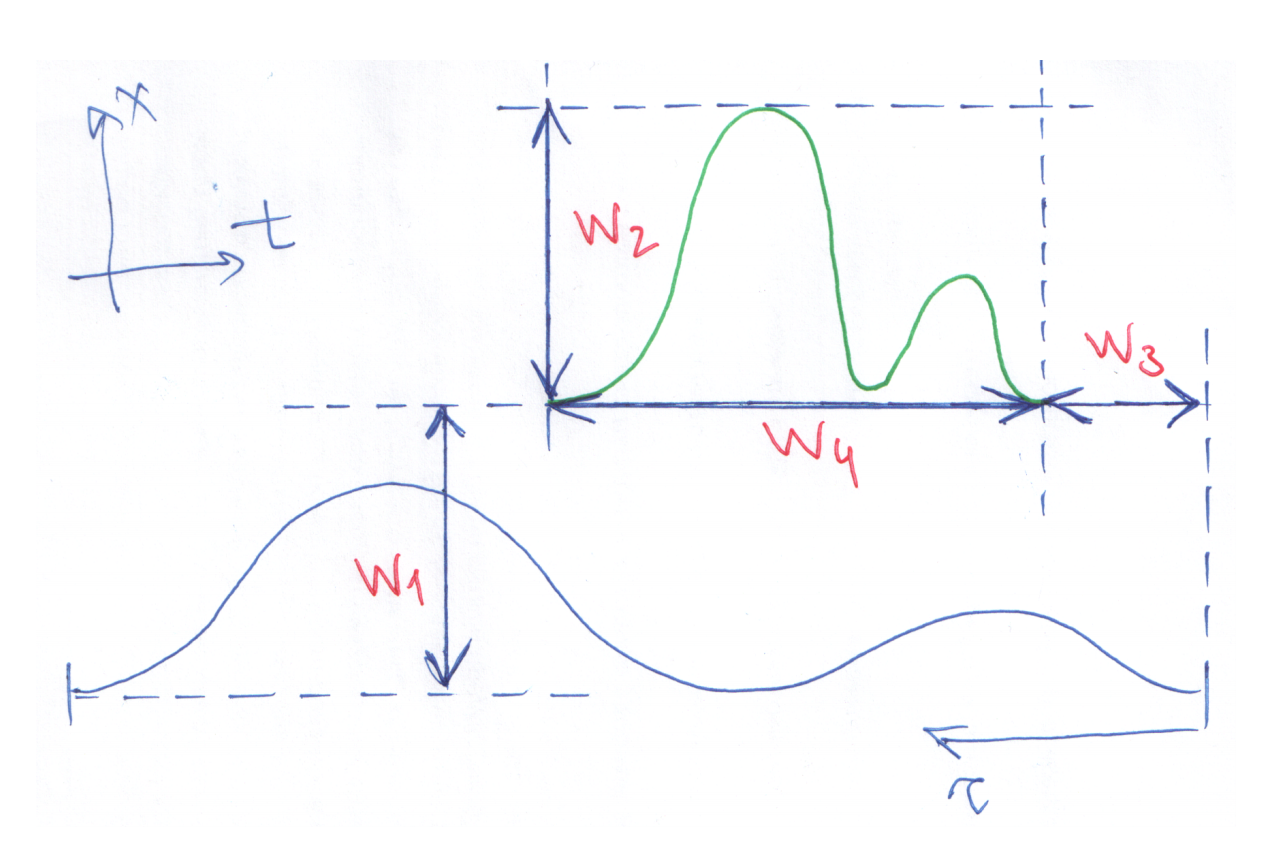
\includegraphics[scale=0.18]{../pics/semor_illustration.png}
                \end{center}
            \end{column}
            \begin{column}{.56\textwidth}
                $$
                g(\bx, \bw) = w_1 + w_2 p(w_3 + w_4t),
                $$
                $$
                w_{\text{SEMOR}} = [\hat{w_1}, \hat{w_2}, \hat{w_3}, \hat{w_4}, \rho].
                $$
            \end{column}
        \end{columns}
    \end{block}
\end{frame}

    % %----------------------------------------------------------------------------------------------------------
\begin{frame}{Построение промежуточной выборки и оптимизация функции потерь
              обобщенной линейной модели}
    \begin{enumerate}
        \item Для каждого $\bh_i \in \bh$ вычисляем
        $$
        [\bz_i^1 \ldots \bz_i^k]^\intercal = [\bh_i(\bx_1) \ldots \bh_i(\bx_k)]
        $$
        \item Конкатенируем вектора параметров $\bz_i = (\bz_1^i \ldots \bz_k^i)$,
        то есть $\bz_i = \bh(\bx_i)$. Получили выборку в промежуточном пространстве $\bZ$.
        \item Минимизируем функции потерь обобщенной линейной модели
        $$
        \hat{\mathbb{\theta}} = \mathrm{arg}\min_{\mathbb{\theta}\in \Theta} L\brs{f(\bZ), \by}.
        $$
    \end{enumerate}
\end{frame}

    % %----------------------------------------------------------------------------------------------------------

    \begin{frame}{Решение задачи: генерация данных}
    \begin{columns} % align columns
        \begin{column}{.4\textwidth}
            \textbf{Данные с акселерометра}: 4 типа движения, частота дискретизации
            100 Гц.

            \textbf{Сегментация}: локальные экстремумы с окном и квантиль по длине
            сегментов.

            \textbf{Нормализация}: приведение к одной размерности с помощью
            кубических сплайнов.

        \end{column}%
        \hfill
        \begin{column}{.6\textwidth}
            \begin{figure}
                \begin{subfigure}[b]{0.48\textwidth}
                    \centering
                    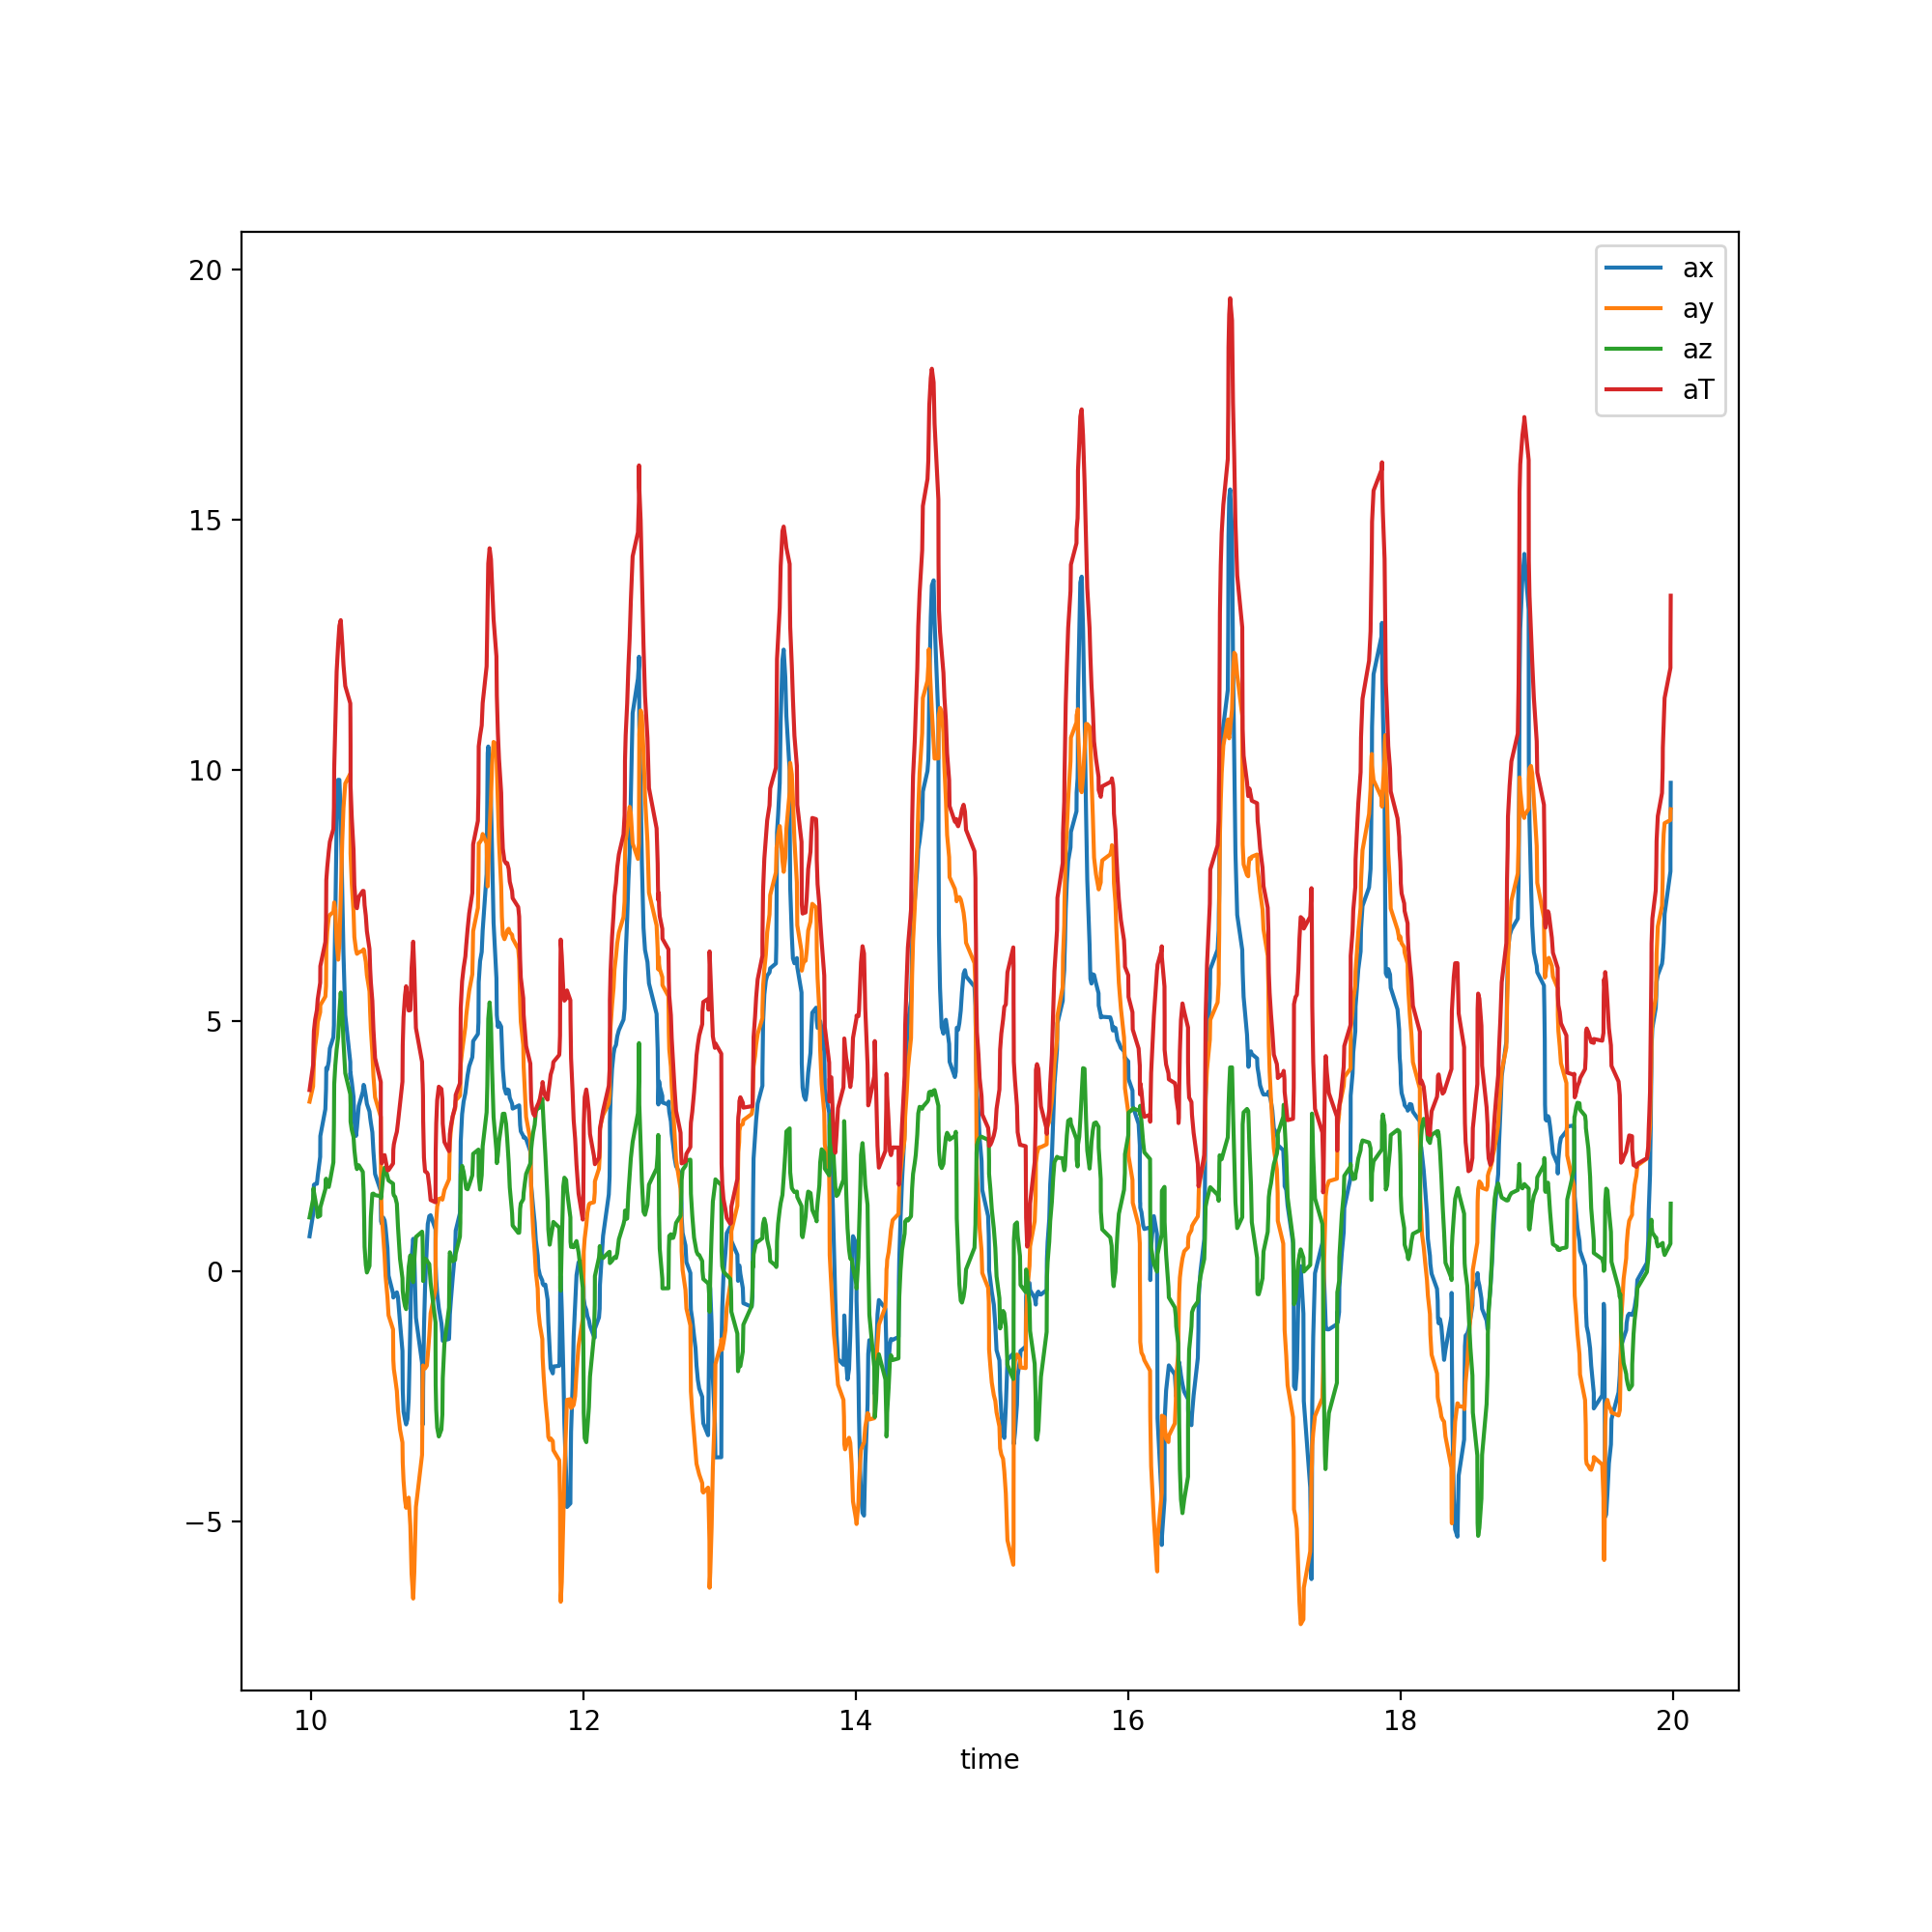
\includegraphics[width=\linewidth]{../pics/raw_walking.png}
                    \caption{Ходьба}
                \end{subfigure}
                \begin{subfigure}[b]{0.48\textwidth}
                    \centering
                    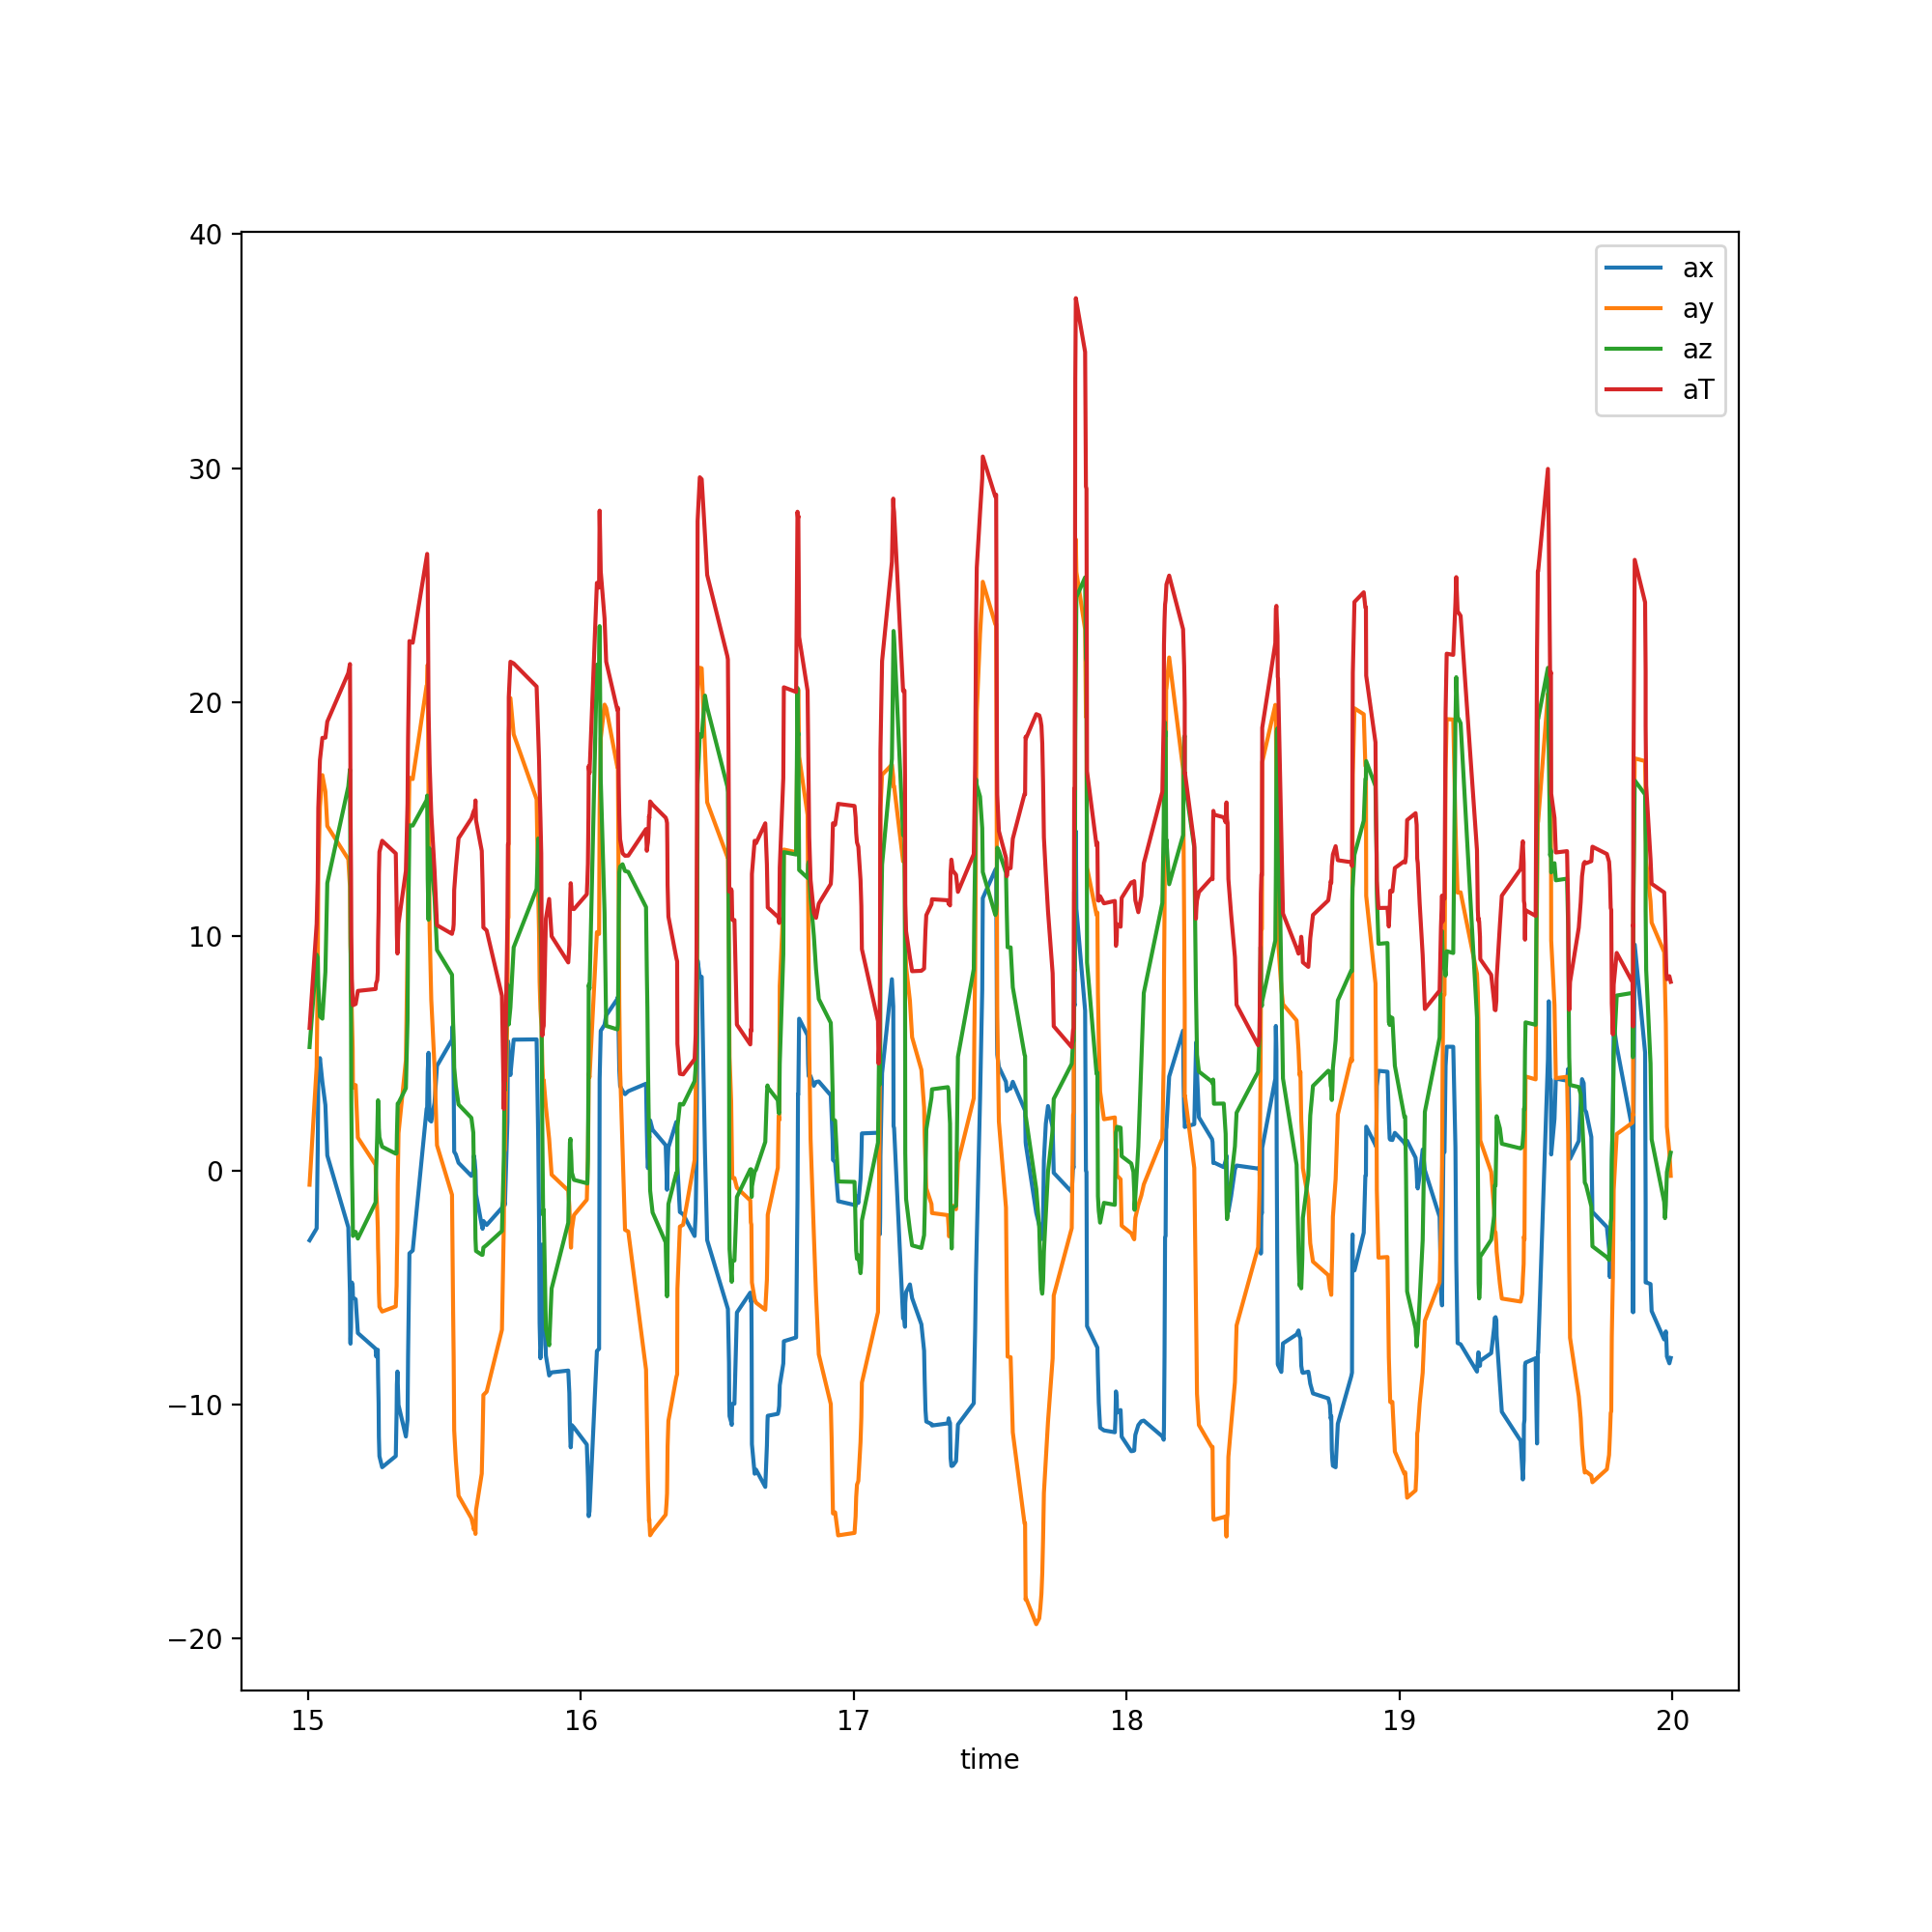
\includegraphics[width=\linewidth]{../pics/raw_run.png}
                    \caption{Бег}
                \end{subfigure}
                \begin{subfigure}[b]{0.48\textwidth}
                    \centering
                    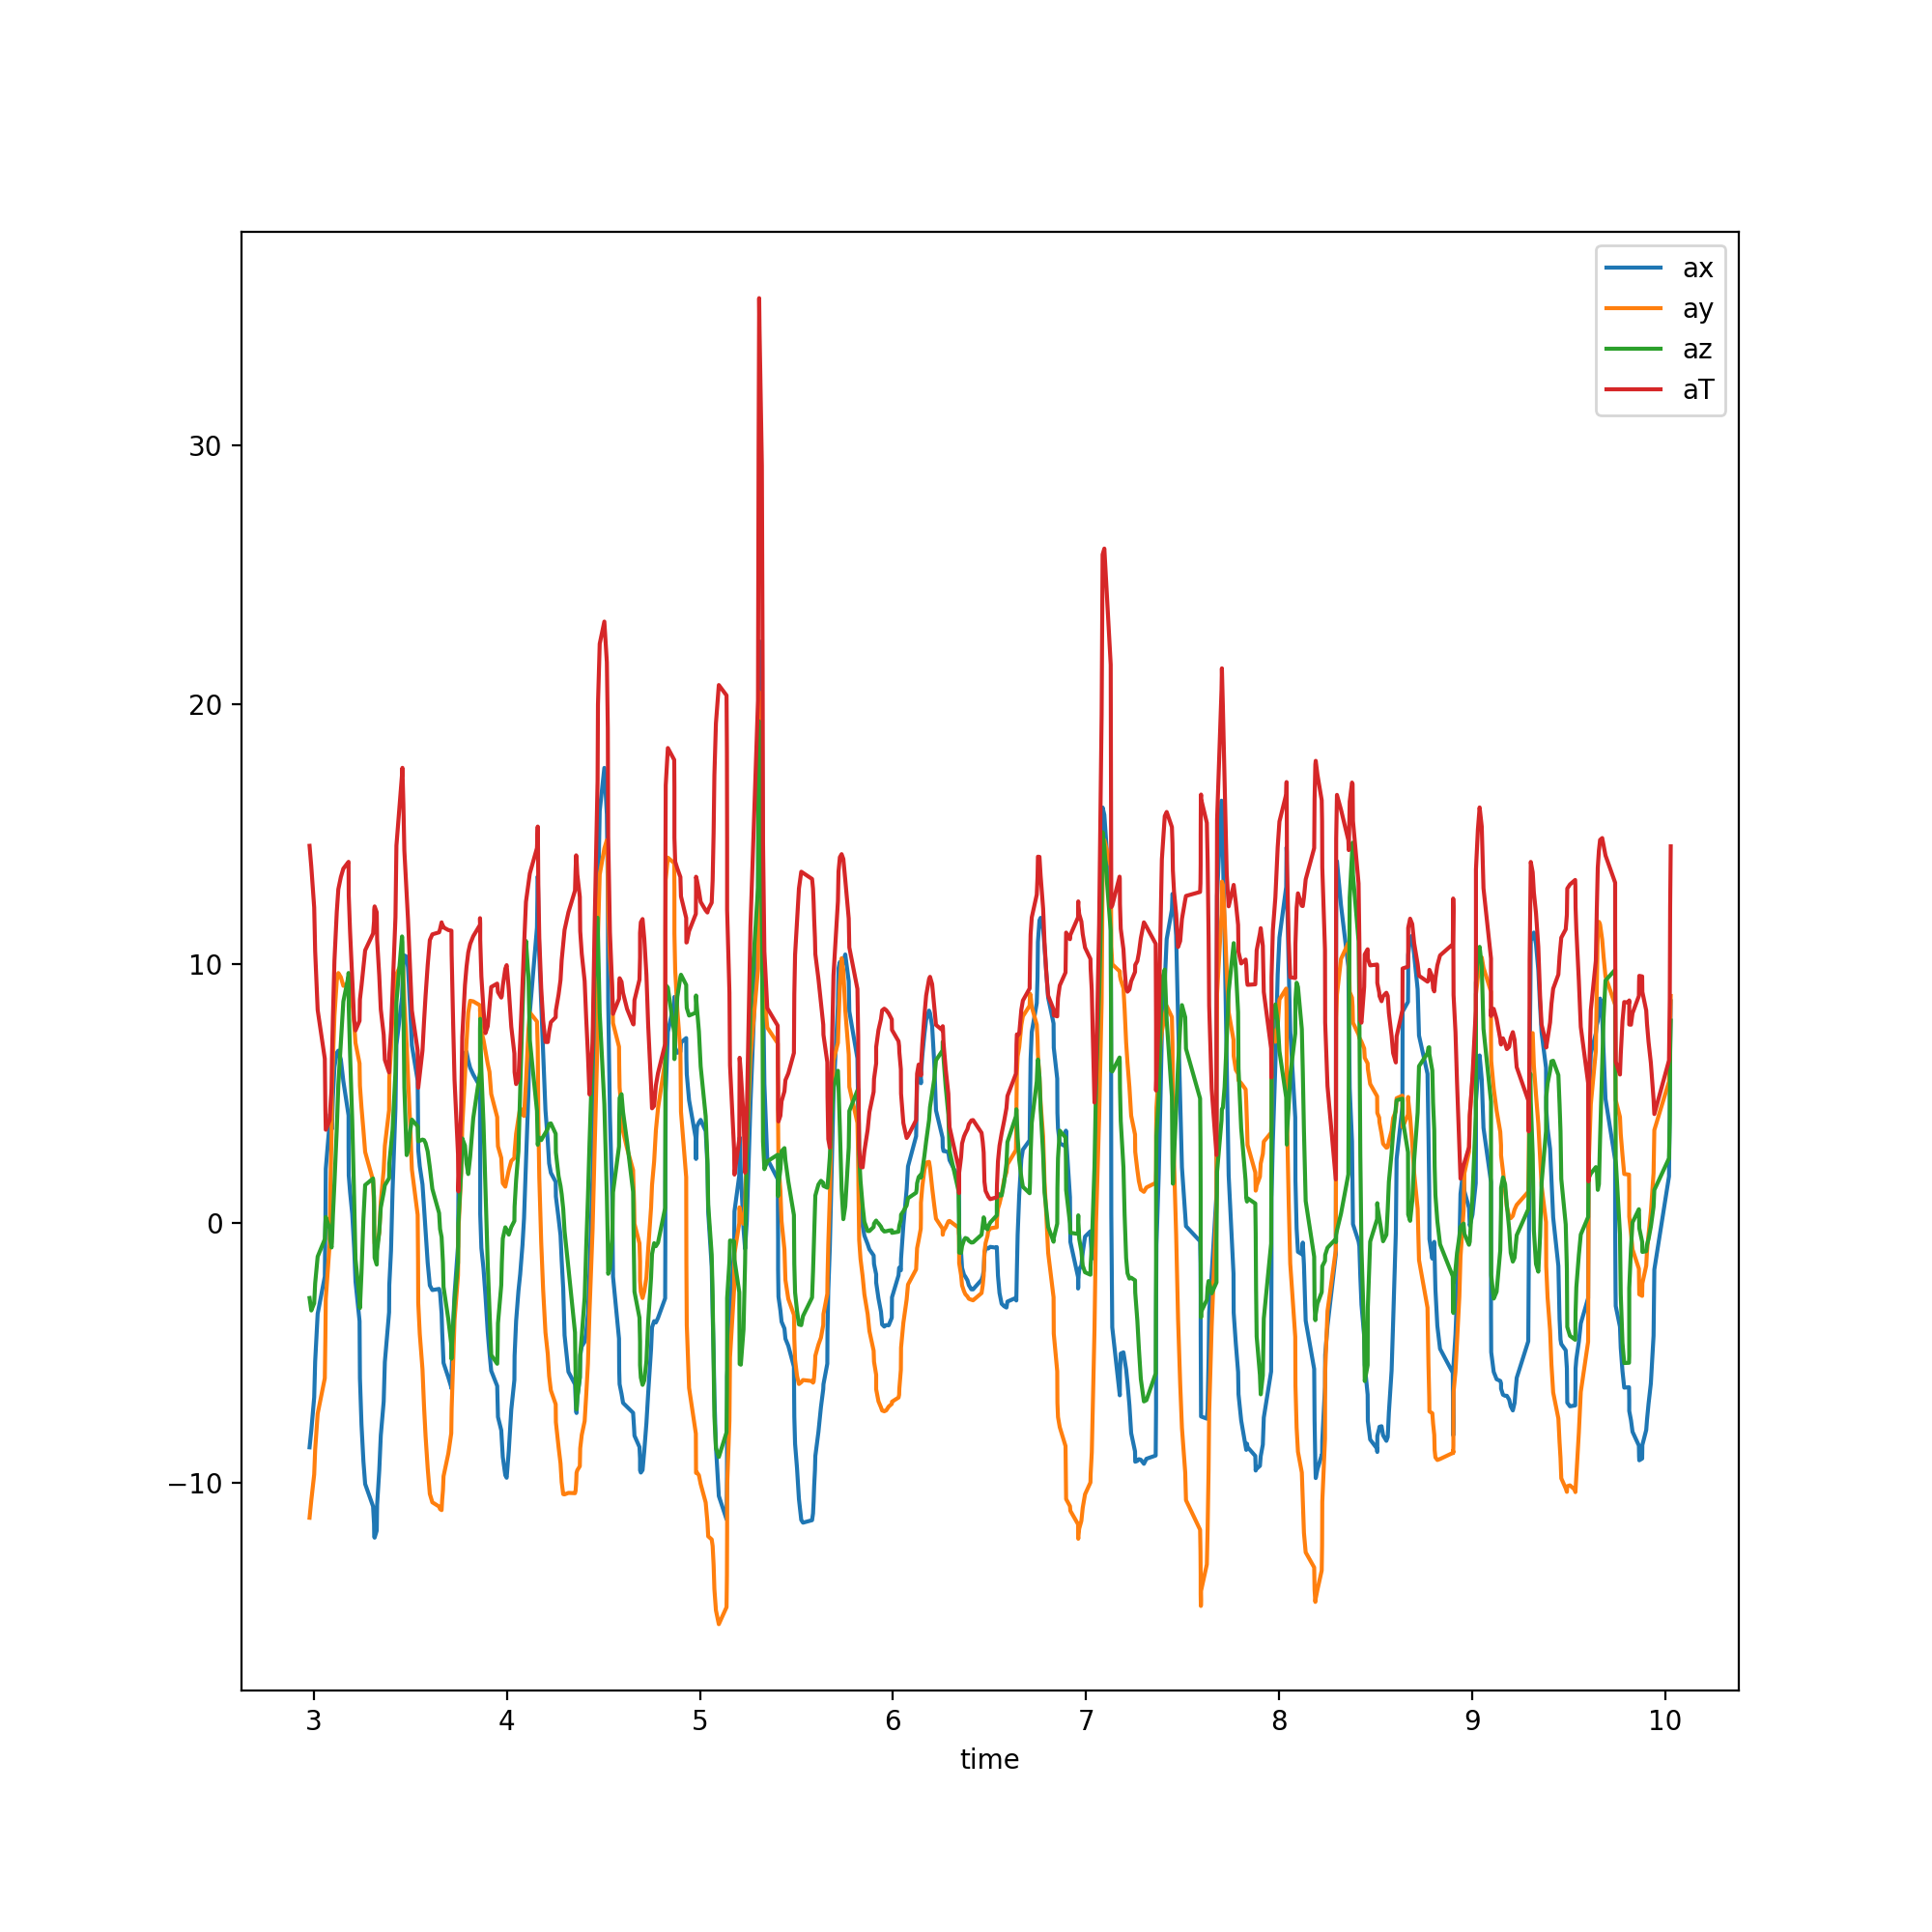
\includegraphics[width=\linewidth]{../pics/raw_go_up.png}
                    \caption{Вверх}
                \end{subfigure}%
                \begin{subfigure}[b]{0.48\textwidth}
                    \centering
                    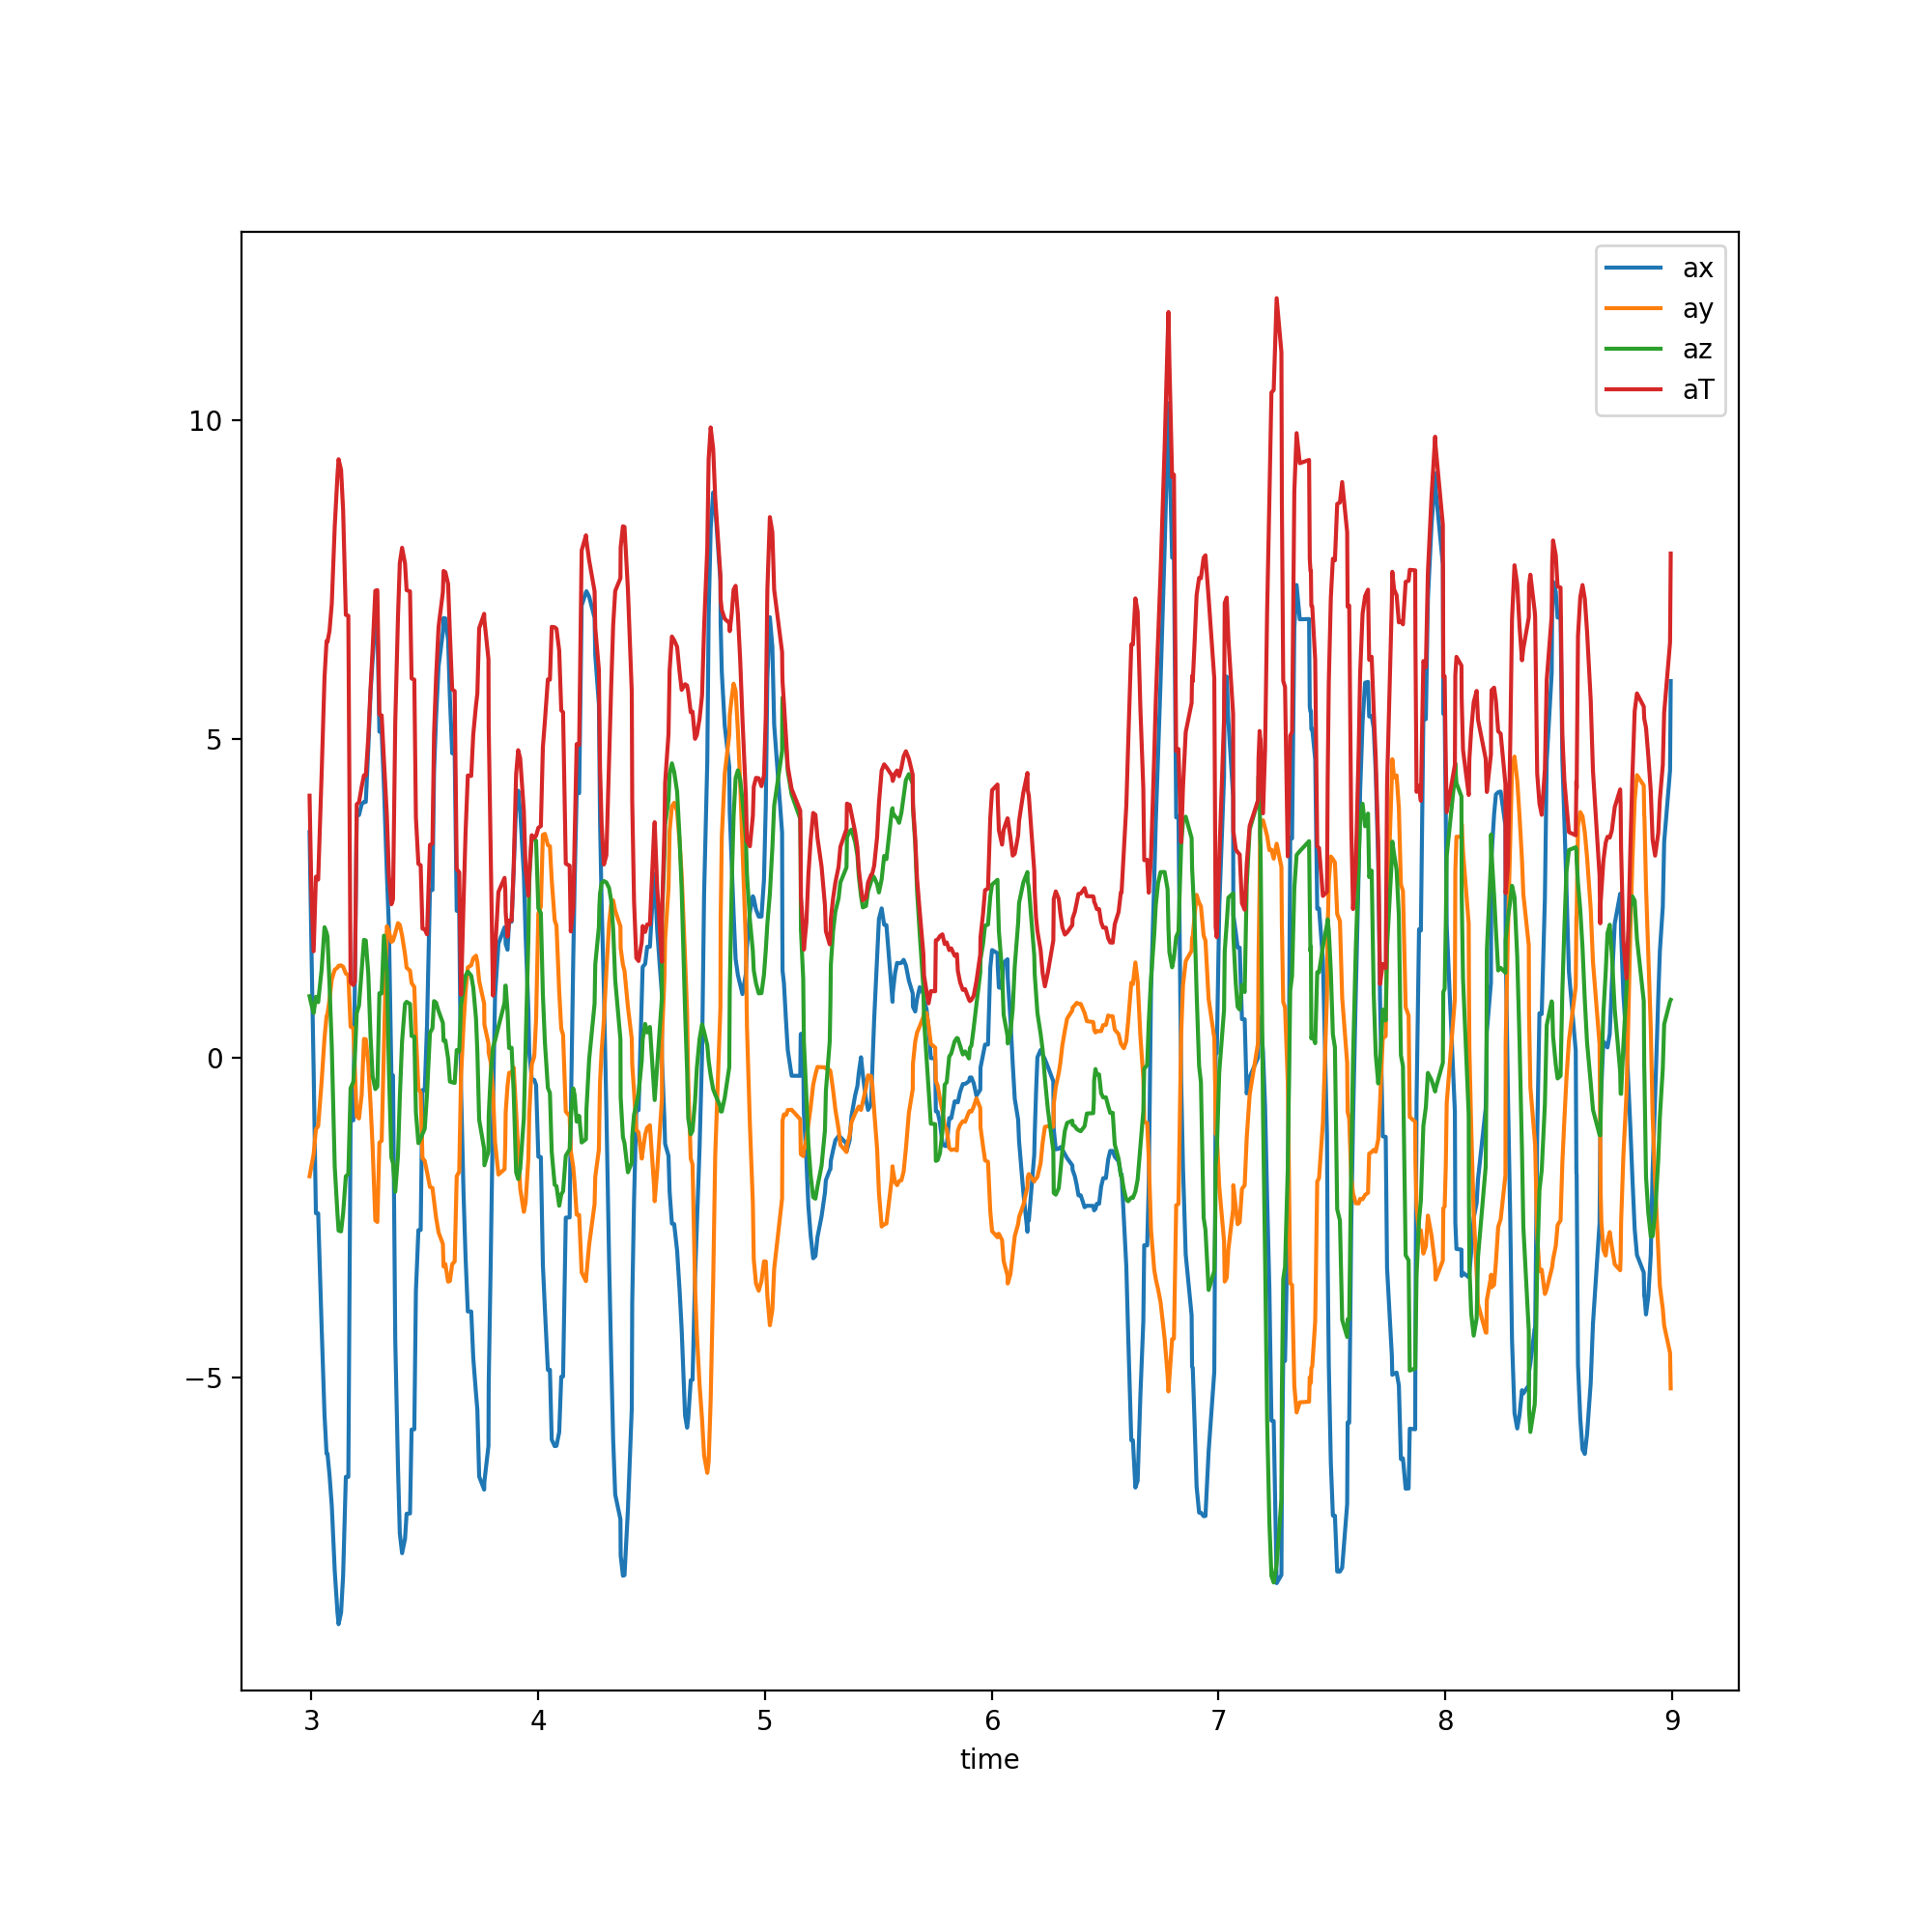
\includegraphics[width=\linewidth]{../pics/raw_go_down.png}
                    \caption{Вниз}
                \end{subfigure}

            \end{figure}
        \end{column}%
    \end{columns}
\end{frame}

    % %----------------------------------------------------------------------------------------------------------

\begin{frame}{Решение задачи: проверка гипотезы простоты выборки}
    \textbf{Тесты простоты выборки}: ($T$-тест) $\mathbb{E} \eps = 0, D \eps = \mathrm{const}$, а также

    \begin{columns}[T] % align columns
        \begin{column}{.48\textwidth}
        анализ унимодальности распределений

    \begin{figure}[ht]
        \centering
          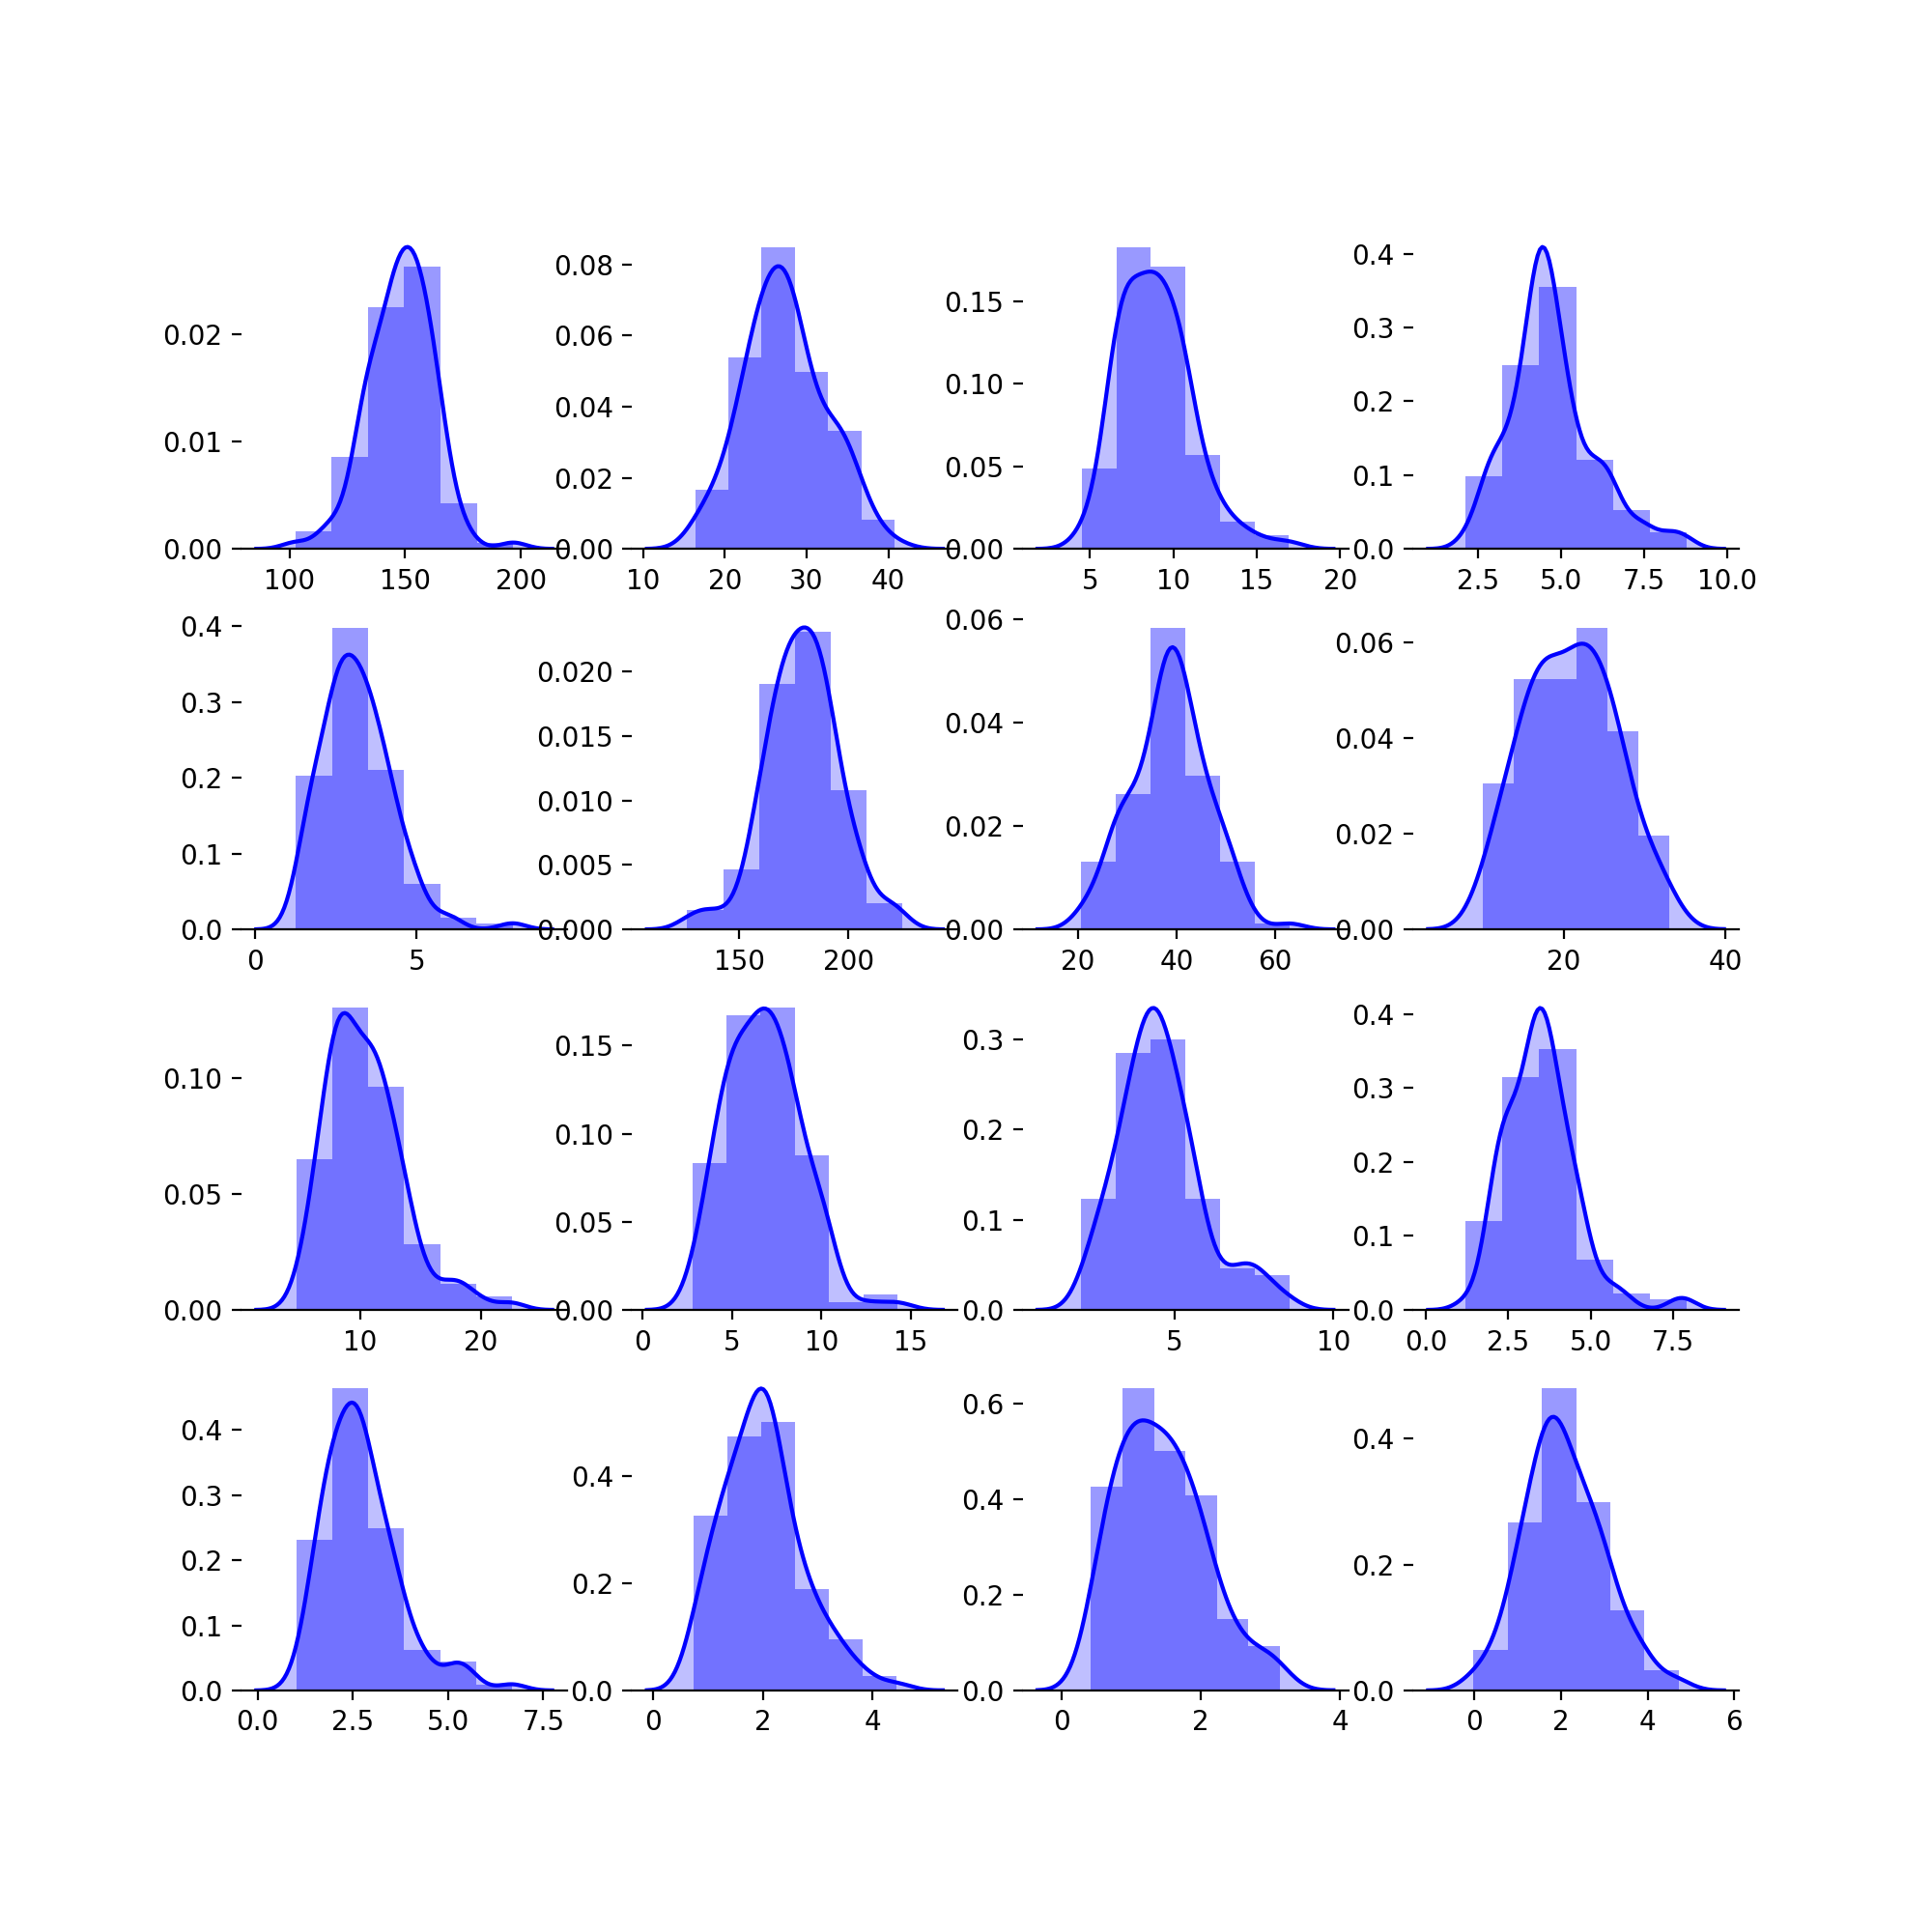
\includegraphics[width=\textwidth]{../pics/features_unimodality_short.png}
    \end{figure}

        \end{column}%
        \hfill%
        \begin{column}{.48\textwidth}
        анализ спектра выборки

    \begin{figure}[ht]
        \centering
          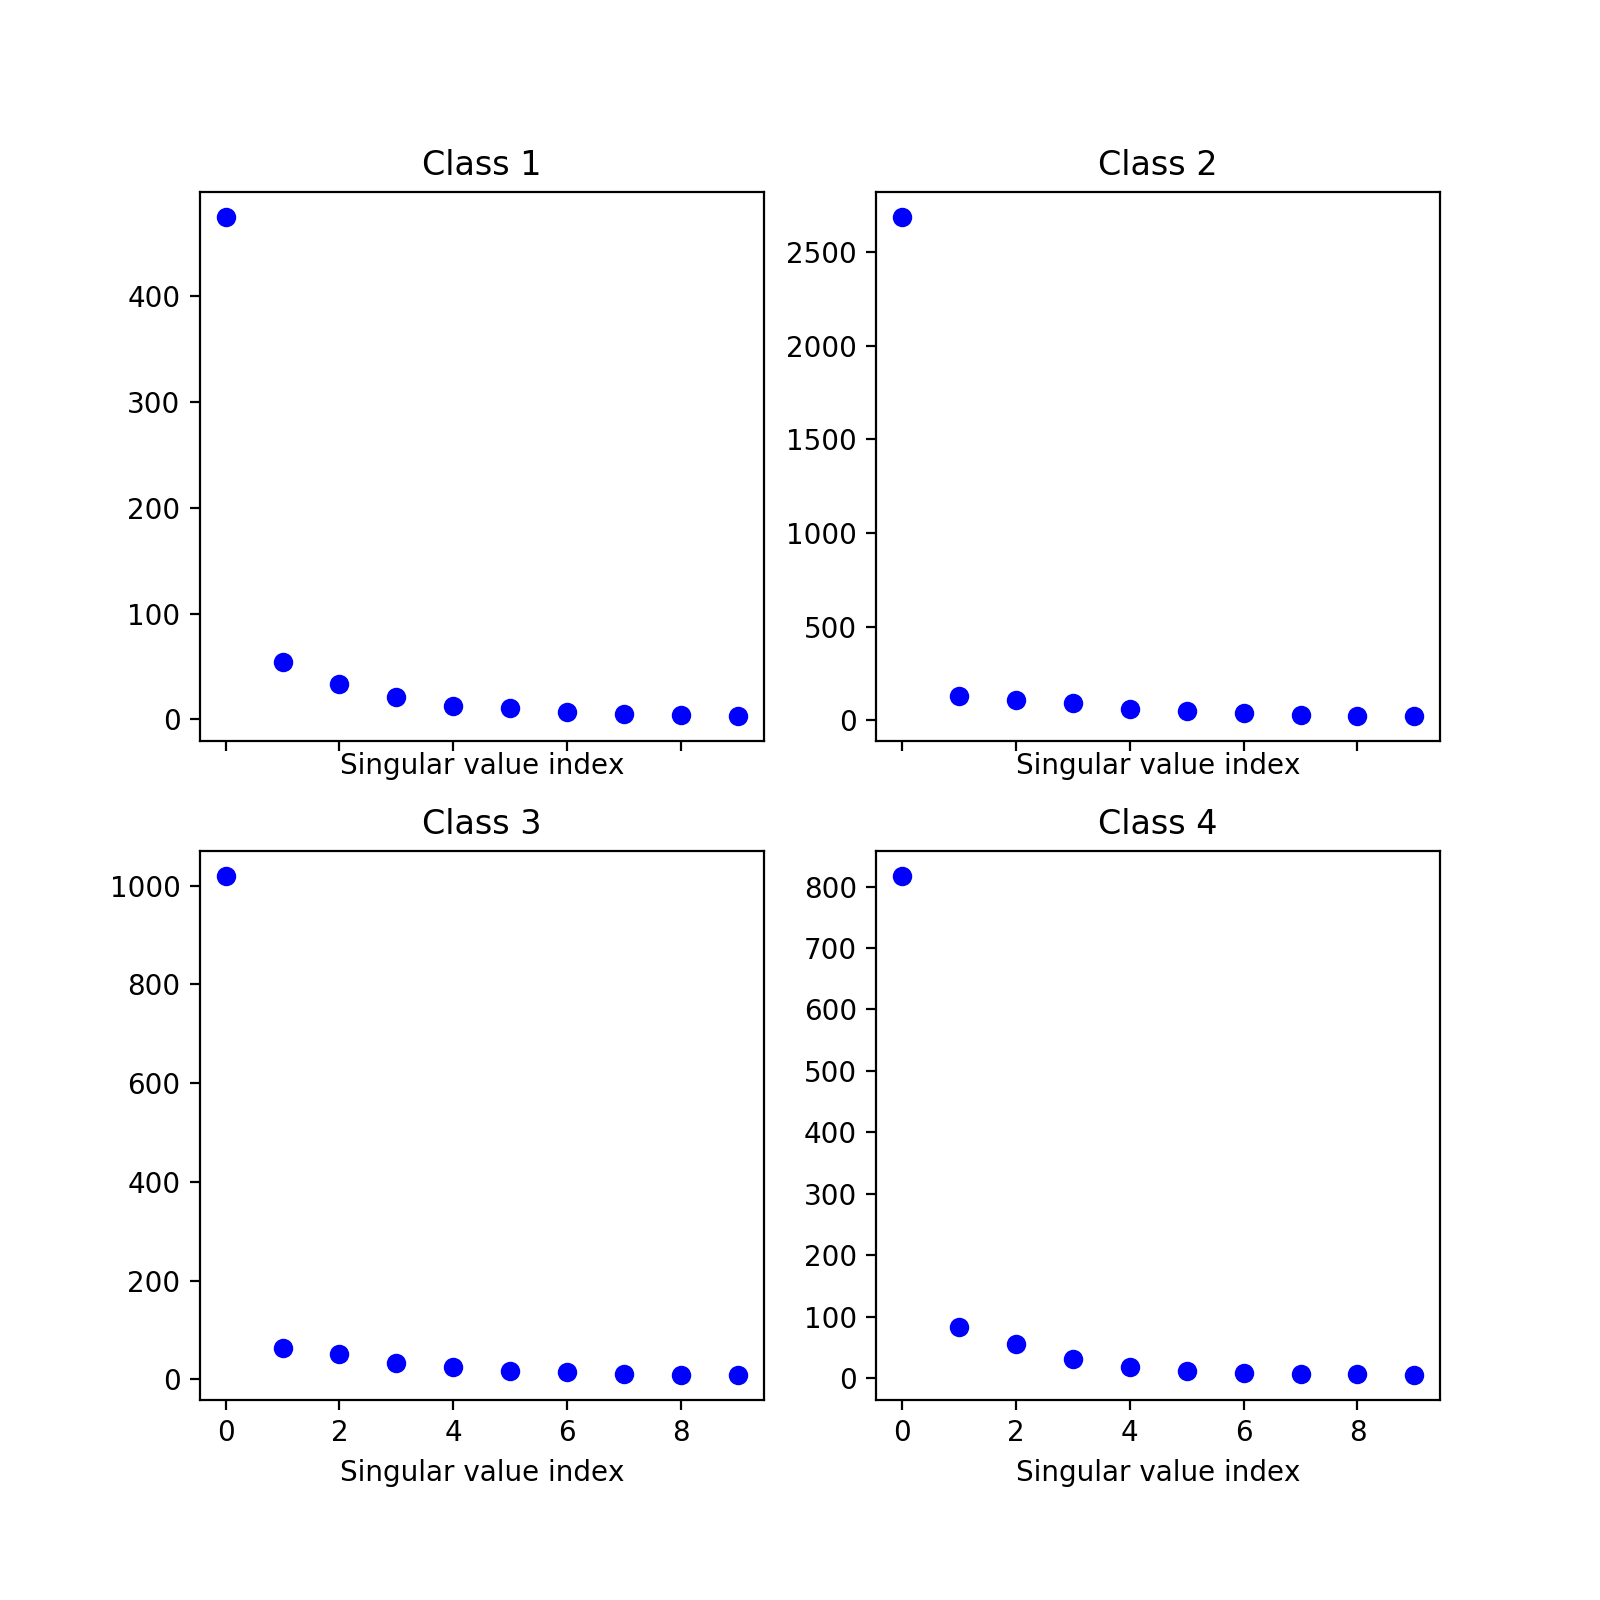
\includegraphics[width=\textwidth]{../pics/sv_analysis.png}
    \end{figure}

        \end{column}%
    \end{columns}
\end{frame}

    % %----------------------------------------------------------------------------------------------------------

\begin{frame}{Обобщенная линейная модель: отбор признаков}
    Сравниваем обобщающую способность обобщенной линейной модели ($\mathrm{GLE}$)
    с универсальной
    моделью при одинаковой сложности.

    Определим сложность модели как
    $$
        \mathrm{Comp}(\mu) = \#|\text{neurons in the hidden layer}|
    $$

    Отбираем признаки в $(\bZ, \by)$ для обобщенной линейной модели. Логистическая
    регрессия с $L_1$ регуляризацией.
    \begin{columns}
        \begin{column}{.5\textwidth}
            \begin{center}
                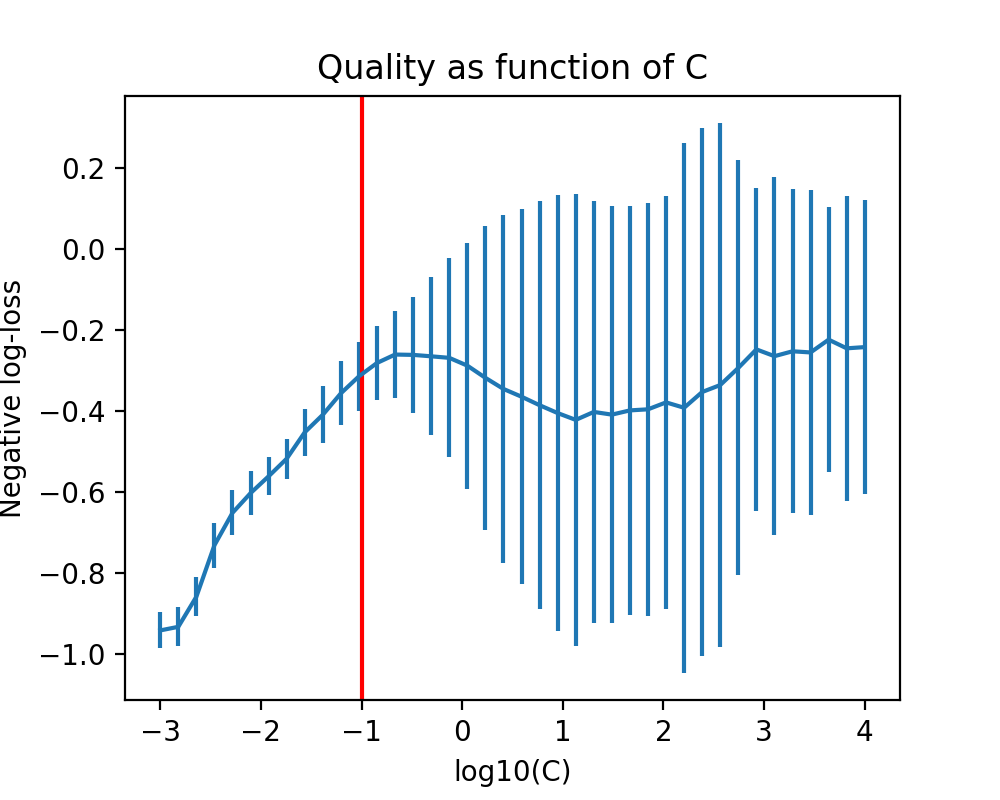
\includegraphics[width=\textwidth]{../pics/lr_quality_C.png}
            \end{center}
        \end{column}
        \begin{column}{.5\textwidth}
            \begin{center}
                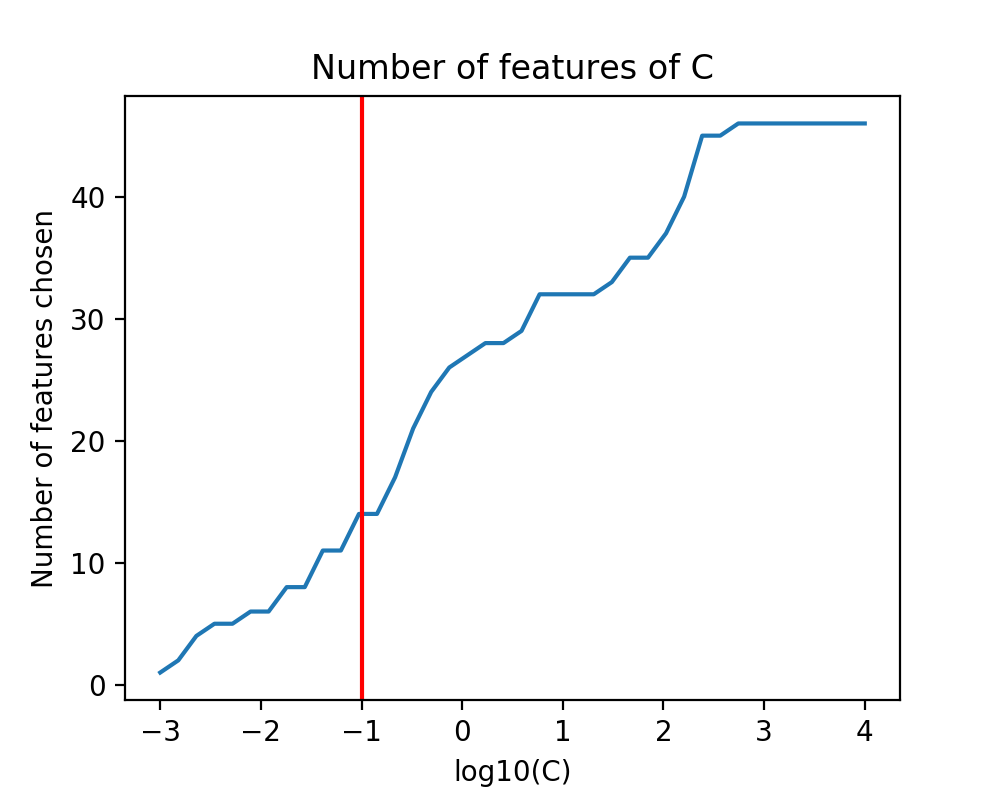
\includegraphics[width=\textwidth]{../pics/lr_n_features_C.png}
            \end{center}
        \end{column}
    \end{columns}
    Выбираем порог $C$, с устраивающей на ошибкой.
\end{frame}

    % %----------------------------------------------------------------------------------------------------------

\begin{frame}{Универсальная модель}

    На выборке $(\bX, \by)$ оптимизируем параметры двуслойной нейронной сети ($\mathrm{NN}$).
    Получаем зависимости
    $$
        L(\mathrm{Comp}), D_L(\mathrm{Comp}).
    $$
    \begin{center}
        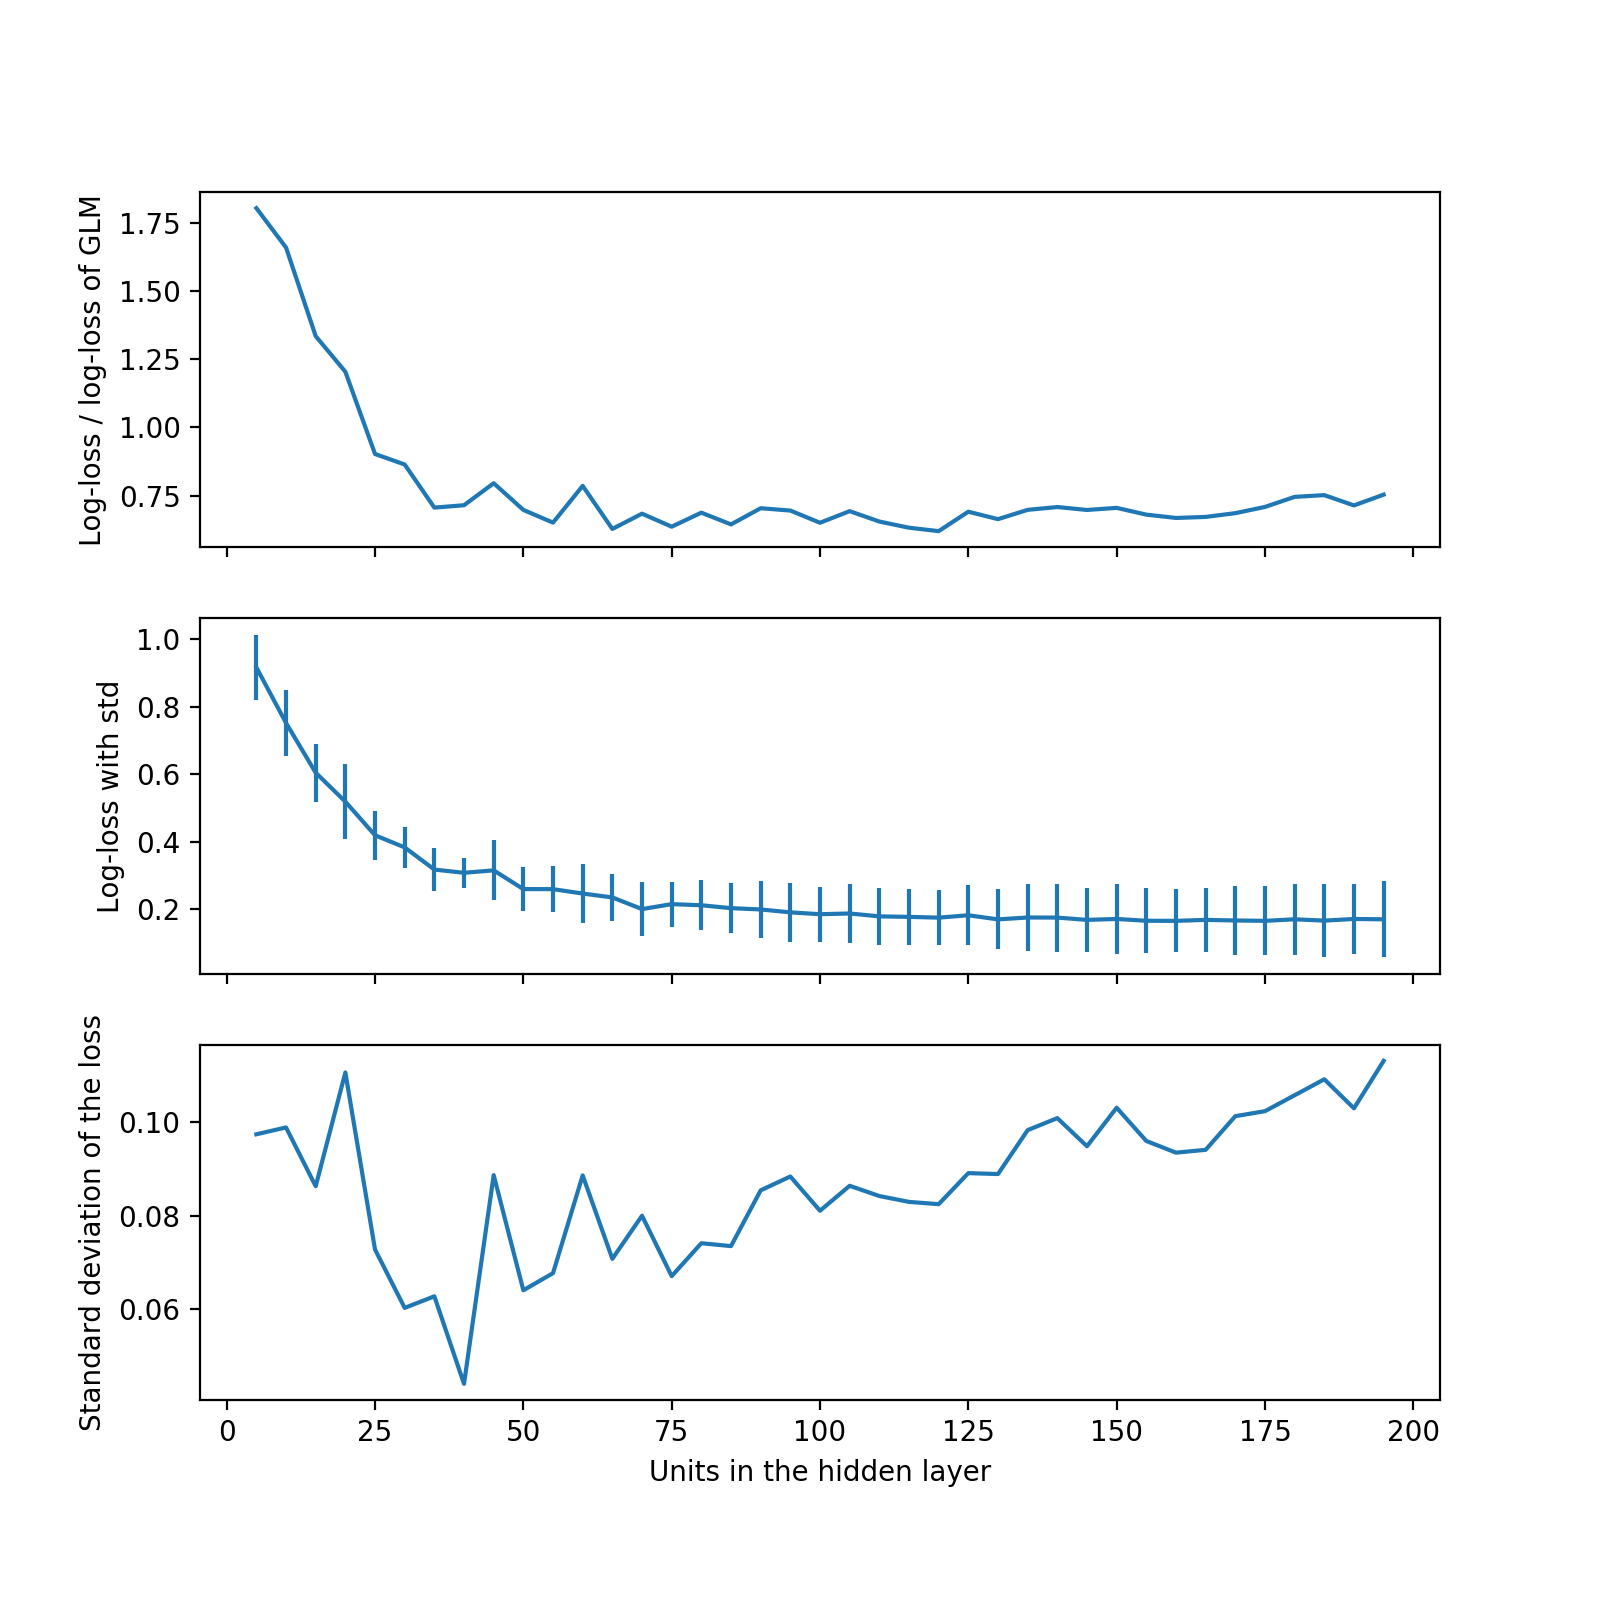
\includegraphics[width=\textwidth]{../pics/loss_and_std_of_n_units_reg.png}
    \end{center}
\end{frame}

    % %----------------------------------------------------------------------------------------------------------

\begin{frame}{Сравнение ошибки при разных сложностях универсальной модели}
    \vspace{-3 mm}
    \begin{figure}[ht]
        \centering
          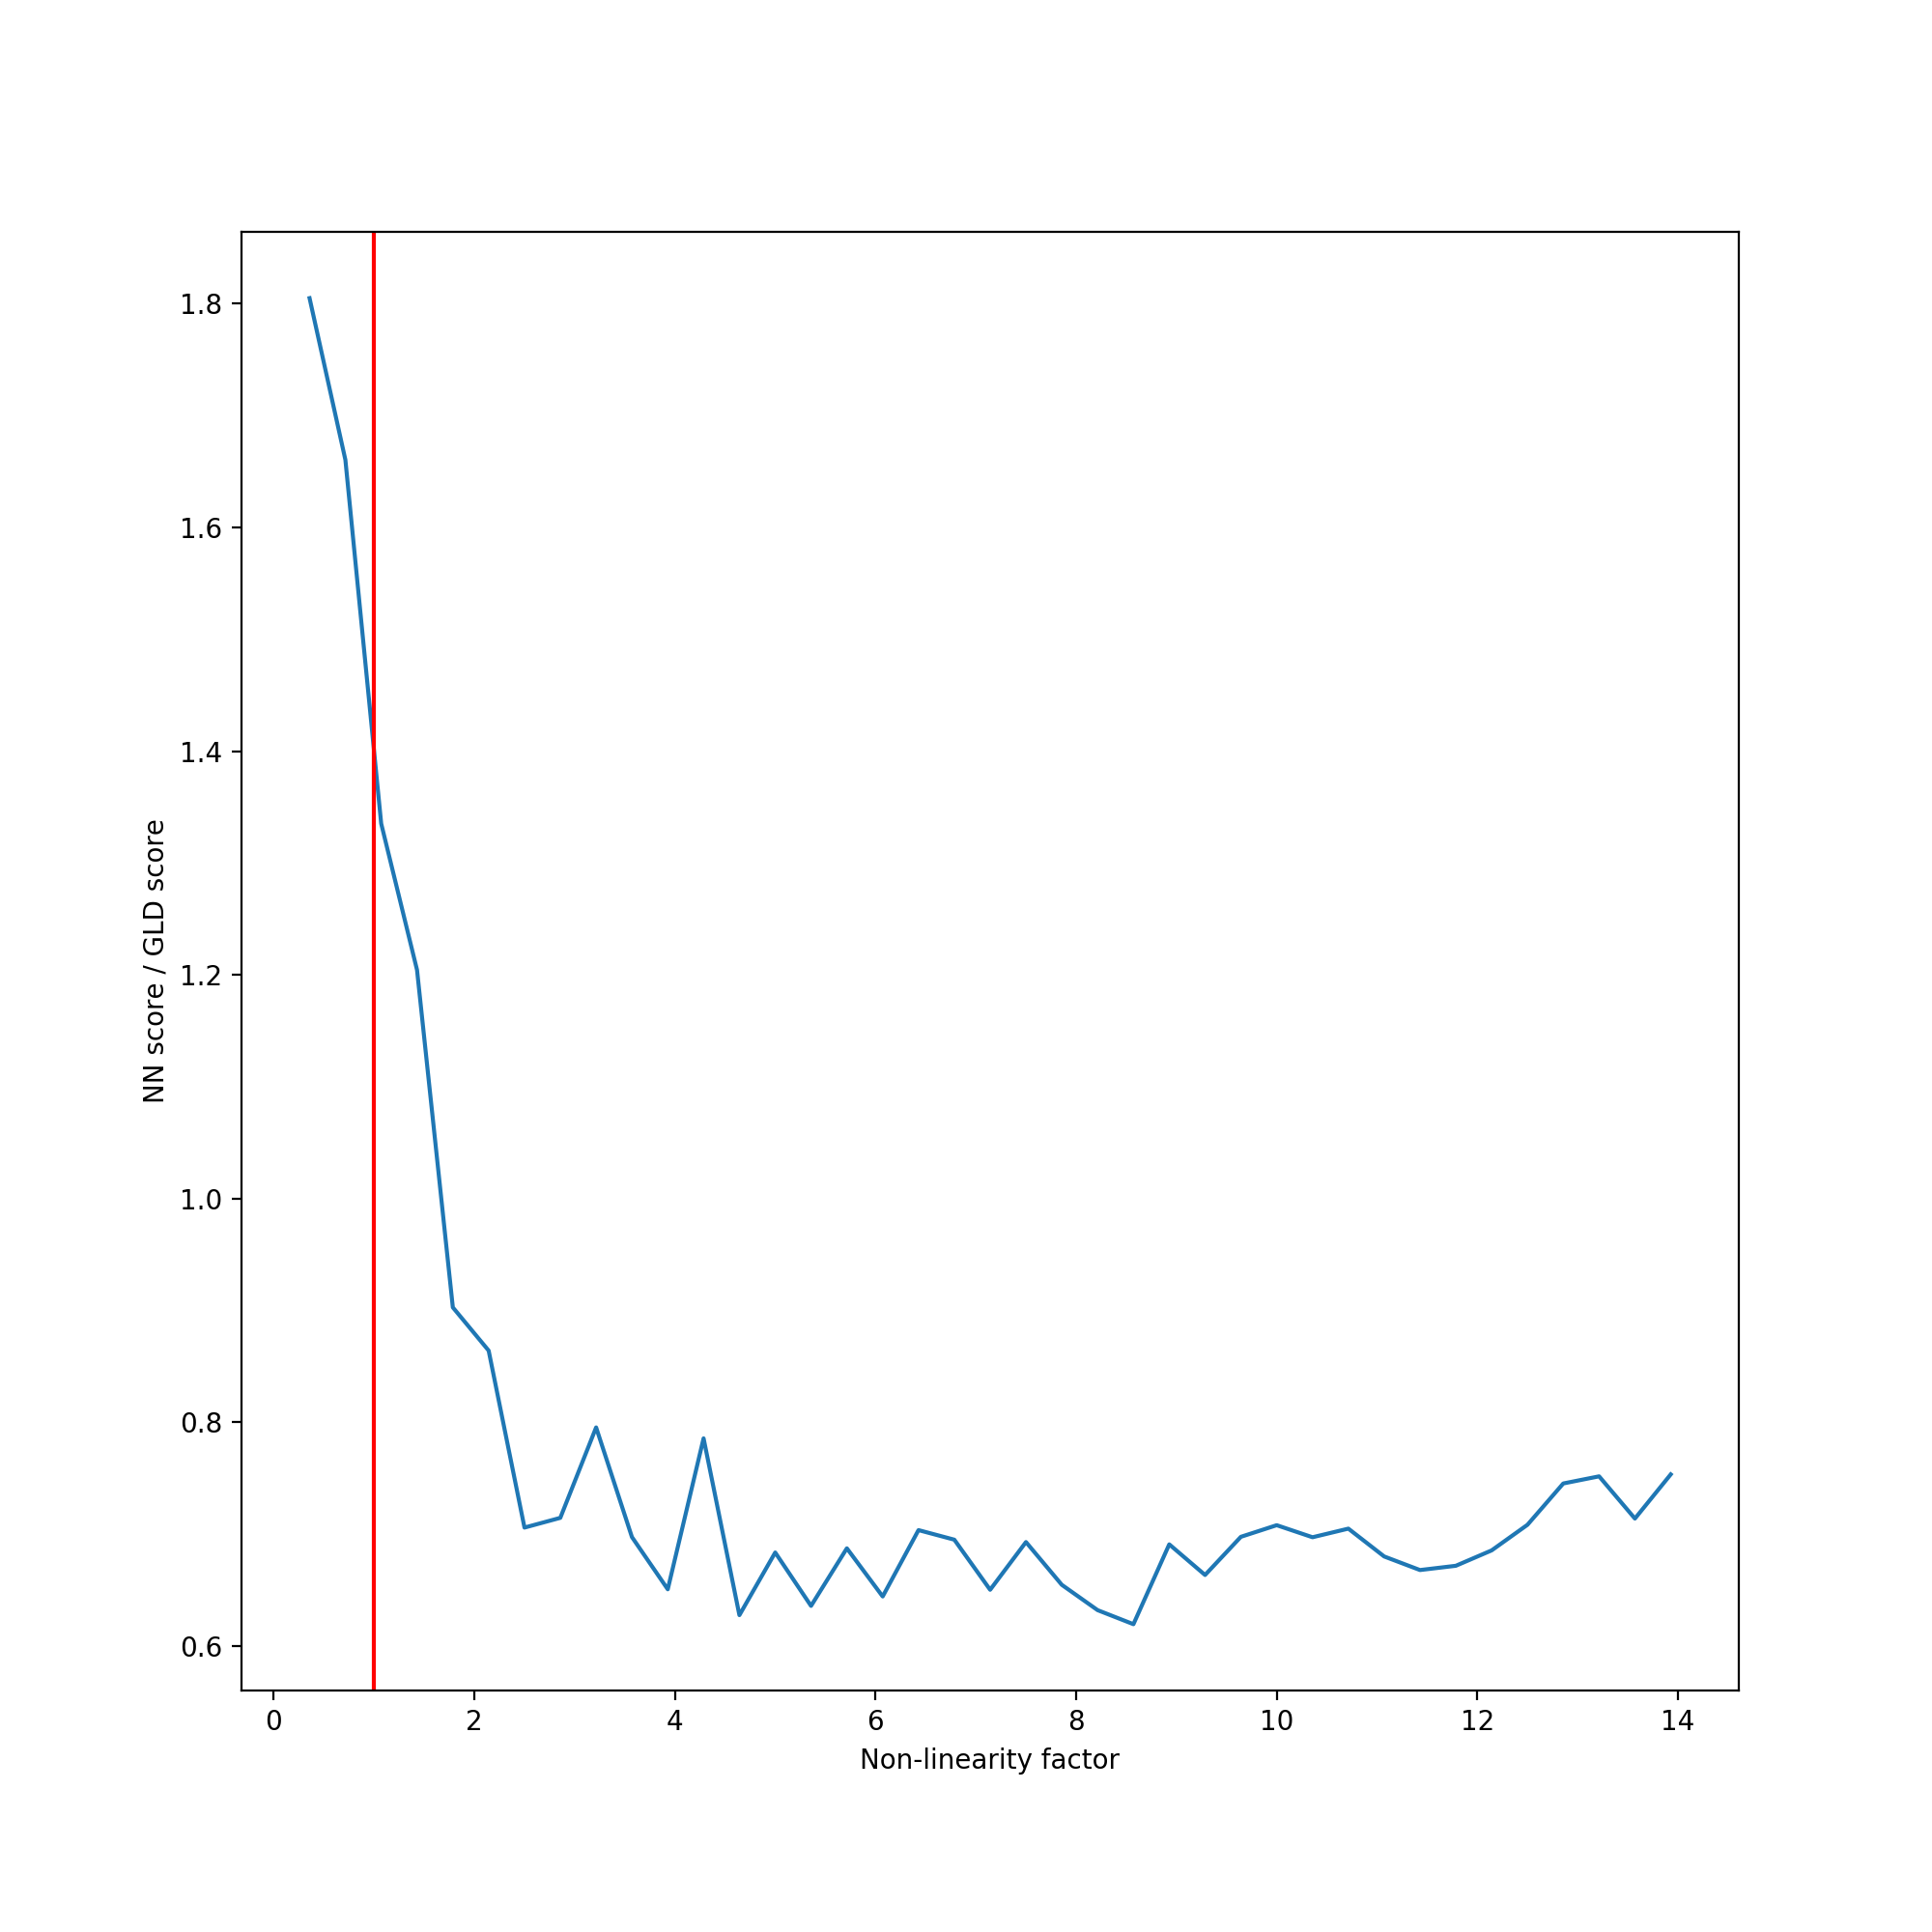
\includegraphics[width=\textwidth]{../pics/loss_and_std_of_nl_factor.png}
          \caption{Отношение ошибок от отношения сложностей}
    \end{figure}
    Результат: при $\mathrm{Comp}(\mathrm{GLE}) = \mathrm{Comp}(\mathrm{NN})$,
    имеем $\frac{L(\mathrm{NN})}{L(\mathrm{GLE})} = 1.4,
    \frac{D_L(\mathrm{NN})}{D_L(\mathrm{GLE})} > 1$.
\end{frame}


\begin{frame}{Выводы}
    \begin{itemize}
        \item Предлоджен тест простоты выборки в промежуточном пространстве признаковых
        описаний, способ простроения обобщенной линейной модели на этих признаках
        а также способ оценки ее обобщающей способности по сравнению с универсальными моделями.
        \item Исследованы статистические свойства промежуточного пространства
        признаковых описаний временных рядов. Выборка в промежуточном пространстве простая,
        а аппроксимирующие ее линейная модель являются адекватной.
        \item GLM адекватнее разделяет выборку чем универсальная модель, то есть
        при одинаковой сложности обеспечивает более высокое качество и меньше переобучается.
    \end{itemize}
\end{frame}

    % \begin{frame}{Постановка задачи}
    % \begin{block}{\bf Задача ретроспективного прогноза}
    % По известному отрезку ряда $\mathbf{x}=[x_1, ..., x_T]^\intercal$ построить прогноз $\hat{x}_{T+1}$ ряда в момент времени $T+1$.
    % \end{block}
    % \begin{block}{\bf Прогноз суперпозицией моделей}
    % $$\hat{x}_{T+1} = f\circ g(\mathbf{\hat{w}}, x_T, x_{T-1}, \ldots, x_1)$$
    % $$f, g\in \mathcal{F}$$
    % $\mathcal{F}$ -- семейство моделей-кандидатов, $\hat{w}\in\mathbb{R}^n$
    % \end{block}
    % \end{frame}

    % %----------------------------------------------------------------------------------------------------------

    % \begin{frame}{Критерий качества}
    % \begin{block}{\bf Предположения}
    % $$\varepsilon_{t} = x_t - \hat{x}_t,\quad\varepsilon_{t}\sim X, \quad \mathsf{E}(\varepsilon_t) \neq 0,\quad \mathsf{D}(\varepsilon_t) = \sigma^2$$
    % $X$ -- асимметричное распределение (пример: обратное распределение Гаусса).
    % \end{block}
    % \begin{block}{\bf Метрики качества прогноза}
    % $$\mathrm{MAPE} = \frac{1}{T}\sum_{t=1}^T \left|\frac{\varepsilon_t}{x_t}\right|, \quad \mathrm{MSE} = \frac{1}{T}\sum_{t=1}^T \varepsilon_t^2.$$
    % \end{block}
    % \begin{block}{\bf Оптимальная суперпозиция}
    % $$(f,g,\mathbf{\hat{w}})=\argmin_{f\in\mathcal{F},~g\in\mathcal{F},~\mathbf{\hat{w}}} \mathrm{MSE}(f\circ g(\mathbf{\hat{w}},x_T,x_{T-1},\ldots,x_1))$$
    % \end{block}
    % \end{frame}

    % %----------------------------------------------------------------------------------------------------------

    % \begin{frame}{Алгоритм блочного прогноза}

    % \begin{block}{\bf Алгоритм последовательного прогноза с накоплением}
    % $x_{T+1}$ считается по известному фрагменту ряда $x_1,\ldots,X_T$

    % $x_{T+k+1}$ считается по известному фрагменту ряда $x_1,\ldots,X_T$ и вычисленным значениям прогноза $x_{T+1},\ldots,x_{T+k}$

    % %$k$ называется \textit{запросом прогнозирования}.

    % \end{block}

    % \begin{block}{\bf Проблема}
    % Учёт качества прогнозирования на запросах, превышающих единицу, при выборе оптимальной суперпозиции.
    % \end{block}

    % \begin{block}{\bf Решение}
    % \begin{itemize}
    % \item Тестовая часть выборки разбивается на блоки длины $r$,
    % \item В пределах блока используется алгоритм прогнозирования с накоплением,
    % \item При переходе к следующему блоку значения предыдущего заменяются на истинные значения из тестовой выборки.
    % \end{itemize}
    % \end{block}

    % \end{frame}

    % %----------------------------------------------------------------------------------------------------------

    % \begin{frame}{Семейство моделей-кандидатов}
    % Состав семейства $\mathcal{F}$ моделей-кандидатов:
    % \begin{enumerate}
    % \item{Экспоненциальное сглаживание (параметр сглаживания $\alpha$),}
    % \item{Метод Кростена (параметр сглаживания $\alpha$),}
    % \item{Ядерное сглаживание (ядро, ширина окна),}
    % \item{Гусеница <<SSA>> (ширина окна, число спектральных компонент),}
    % \item{ARIMA (p,d,q),}
    % \item{Квантильная регрессия (функция штрафа),}
    % \item{LSTM (длина истории, эвристика).}
    % \end{enumerate}
    % В скобках указаны перебираемые по сетке структурные параметры.
    % \end{frame}

    % %----------------------------------------------------------------------------------------------------------

    % \begin{frame}{Зависимость качества от структурных параметров}
    % \makebox[\textwidth][c]{\includegraphics[width=\textwidth]{airline_10/hyperparameters}}
    % \end{frame}

    % %----------------------------------------------------------------------------------------------------------

    % \begin{frame}{Прогнозы основных моделей}
    % \makebox[\textwidth][c]{\includegraphics[width=\textwidth]{german_10/models_demo}}
    % \end{frame}

    % %----------------------------------------------------------------------------------------------------------

    % \begin{frame}{Матрица качества суперпозиций}
    % % FIXME: нормальная ошибка, а не log MSE
    % \makebox[\textwidth][c]{\includegraphics[width=\textwidth]{german_10/superposition}}
    % \end{frame}

    % %----------------------------------------------------------------------------------------------------------

    % \begin{frame}{Эмпирическая функция распределения ошибки}
    % \makebox[\textwidth][c]{\includegraphics[width=0.9\textwidth]{german_10/remainders}}
    % \end{frame}

    % %----------------------------------------------------------------------------------------------------------

    % \begin{frame}{Зависимость ошибки от горизонта прогнозирования}
    % % FIXME: линия для правила сломанной трости
    % \makebox[\textwidth][c]{\includegraphics[width=0.9\textwidth]{railroads_10/error_vs_horizon}}
    % \end{frame}


    % %----------------------------------------------------------------------------------------------------------

    % \begin{frame}{Зависимость ошибки от скоса распределения}
    % % FIXME: линия для правила сломанной трости
    % \makebox[\textwidth][c]{\includegraphics[width=0.9\textwidth]{error_vs_skew-eps-converted-to}}
    % \end{frame}

    % %----------------------------------------------------------------------------------------------------------

    % \begin{frame}{Результаты}
    % \begin{itemize}
    % \item Рассмотрены суперпозиции базовых алгоритмов (экспоненциальное сглаживание, метод Кростена, SSA, ARIMA, квантильная регрессия, LSTM).
    % \item Построены матрицы качества суперпозиций, распределение остатков модели, определён горизонт прогнозирования.
    % \item Показано, что использование суперпозиций может повышать качество прогноза.
    % \item Исследована зависимость ошибки от степени асимметричности распределения шумовых остатков: с ростом асимметричности суперпозиции достигают меньшей ошибки, чем базовые модели.
    % \end{itemize}
    % \end{frame}

    % %----------------------------------------------------------------------------------------------------------

    % \begin{frame}{Спасибо за внимание}
    % \end{frame}

    %----------------------------------------------------------------------------------------------------------

    \end{document}
